\documentclass[12pt,a4paper]{report}
\usepackage{vntex} % Tiếng Việt
\usepackage{graphicx} % Chèn hình ảnh
\usepackage{fancyhdr} % Gói hỗ trợ tạo header và footer fancy
\usepackage{changepage} % Thay đổi lề

% Chèn code
\usepackage{listings} % Thêm gói listings để chèn code
\usepackage{xcolor} % Màu cho code
\lstset{
    language=Matlab,
    basicstyle=\footnotesize\ttfamily,
    numbers=none,
    numberstyle=\tiny\color{gray},
    stepnumber=1,
    numbersep=0.01pt,
    tabsize=2,
    breaklines=true,
    breakatwhitespace=false,
    xleftmargin=0cm, % for line numbers
    framexleftmargin=0cm, % for code frame
    keywordstyle=\color{blue},
    commentstyle=\color{green},
    stringstyle=\color{orange},
    frame=single,
    rulecolor=\color{black},
    basicstyle=\ttfamily,
}

% Footnote and References
\usepackage[style=numeric,backend=biber]{biblatex} % Sử dụng gói biblatex
\usepackage{capt-of} %  Footnote trong caption
\usepackage[perpage]{footmisc} % Đánh số lại chú thích mỗi trang

% Thiết lập bảng
\usepackage{array} % Gói hỗ trợ các bảng phức tạp
\usepackage{tabularx}
\usepackage{longtable} % Tạo bảng qua nhiều trang
\usepackage{cellspace}
\usepackage{diagbox} % Gói hỗ trợ tạo các ô chéo trong bảng
\usepackage{multirow}

% Thiết lập công thức toán học
\usepackage{amsmath} % Gói hỗ trợ các công thức toán học
\usepackage{amsfonts} % Gói hỗ trợ các ký hiệu toán học
\usepackage{amssymb} % Gói hỗ trợ các ký hiệu toán học
\usepackage{graphicx} % Gói hỗ trợ chèn hình ảnh
\usepackage{bm} % Chữ in đậm trong công thức toán 

% Thiết lập khác
\usepackage{tikz}
\usepackage{color}
\usepackage{subcaption}
\usepackage{framed}
\usepackage{float} % Để chèn hình ảnh vào đúng vị trí
\usepackage{fancyvrb} % Đưa dữ liệu dạng nguyên thủy vào


% Thiết lập kích thước
\usepackage{geometry}
\geometry{
    left=3cm,
    right=2cm,
    top=2.5cm,
    bottom=2.5cm,
}
\usepackage{hyperref} %Chèn link
\hypersetup{urlcolor=black,linkcolor=black,citecolor=black,colorlinks=true} % Màu cho các đường nét
\everymath{\color{black}}
\setlength{\headheight}{40pt}
\pagestyle{fancy}

% \addbibresource{references.bib} 

%Header
\fancyhead{} % clear all header fields
\fancyhead[L]{
 \begin{tabular}{rl}
    \begin{picture}(15, 15)(0,0)
    \put(-15, -15){
\includegraphics[width=17mm, height=12mm]{pictures/hcmut.png}}
    %\put(0,-8){\epsfig{width=10mm,figure=hcmut.eps}}
   \end{picture}&
	%
\includegraphics[width=8mm, height=8mm]{hcmut.png} & %
	\begin{tabular}{l}
		\textbf{\bf \ttfamily Trường Đại Học Bách Khoa - ĐHQG TP.Hồ Chí Minh}\\
		\textbf{\bf \ttfamily Khoa Cơ Khí}\\
	\end{tabular} 	
 \end{tabular}
}
\fancyhead[R]{
	{\tiny \bf \quad} % Khoảng trắng nhỏ trong header bên phải
}

%Footer
\fancyfoot{} % clear all footer fields
\fancyfoot[L]{\scriptsize \ttfamily Đồ án chuyên ngành}
\fancyfoot[R]{\scriptsize \ttfamily Trang {\thepage}/70}
\renewcommand{\headrulewidth}{0.3pt}
\renewcommand{\footrulewidth}{0.3pt}

\begin{document}
    \begin{titlepage}   
    \begin{center}
        \vspace*{-2cm} 
        \large
        \textbf{ĐẠI HỌC QUỐC GIA THÀNH PHỐ HỒ CHÍ MINH \\
        TRƯỜNG ĐẠI HỌC BÁCH KHOA\\
        KHOA CƠ KHÍ\\}
        \vspace{0.5cm}
        
\includegraphics[width=70mm, height=70mm]{pictures/hcmut.png} \\
        \rule{\linewidth}{0.5mm}\\
        \vspace{1cm}
        \LARGE
        \textbf{BÀI TẬP LỚN}\\
        \vspace*{0.5cm}
        \Huge
        \textbf{CHI TIẾT MÁY}\\
        \vspace{0.5cm}
        \rule{\linewidth}{0.5mm}\\
        \vspace{0.8cm}
        \vspace{1cm}
        \large
        GVHD: GS. NGUYỄN HỮU LỘC\\[0.5cm]
        HỌ VÀ TÊN SINH VIÊN: VÕ HỮU DƯ\\[0.5cm]
        MSSV: 2210604\\
    \end{center}
        
    \vfill
    \large
    \begin{center}
        TP.HCM, \today
    \end{center}
\end{titlepage}
    \tableofcontents  
    \listoftables
    \listoffigures
    \newpage
    \normalsize
    \chapter{TỔNG QUAN}
    \section{Tìm hiểu về AGV}
    \chapter{LƯA CHỌN PHƯƠNG ÁN}
    \section{Lựa chọn nguyên lý cơ khí}
        \subsection{So sánh các kết cấu cơ khí}
            \hspace*{0.6cm}Yêu cầu:
            \begin{itemize}
                \item Đảm bảo độ bám đường, khó lật khi vào cua với tốc độ cao.
                \item Thuật toán điều khiển đơn giản.
                \item Kết cấu cơ khí vững, nhỏ gọn, ổn định và dễ chế tạo.
                \item Chủ động trong việc chuyển hướng, chuyển hướng tốt. 
            \end{itemize}
        \subsection{So sánh các sơ đồ nguyên lý}
            \hspace*{0.6cm}Xét theo từng sơ đồ nguyên lý đã tìm hiểu trong phần tổng quan, bảng dưới đây 
trình bày ưu và nhược điểm của từng loại sơ đồ:
            \begin{longtable}{|p{4cm}|p{5cm}|p{5cm}|}
                \caption{So sánh các sơ đồ nguyên lý robot} 
                \label{tab:compare_robot_schemes} \\ 
                \hline
                \textbf{Sơ đồ nguyên lý} & \textbf{Ưu điểm} & \textbf{Nhược điểm} \\
                \hline
                \endfirsthead
                \hline
                \textbf{Sơ đồ nguyên lý} & \textbf{Ưu điểm} & \textbf{Nhược điểm} \\
                \hline
                \endhead
                \hline
                \endfoot
                \hline
                \endlastfoot
                Robot Chariot \newline
                \textit{Phương án 1} \newline
                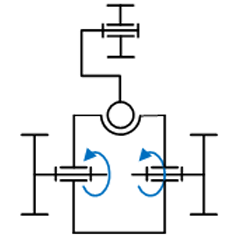
\includegraphics[width=2.5cm]{pictures/chapter2/robot_chariot.png} & 
                - Kết cấu 3 bánh nhỏ gọn, đơn giản \newline
                - Mô hình toán đơn giản, dễ điều khiển & 
                - Khi vào cua dễ bị lật. \newline
                - Khả năng bám đường kém. \newline
                - Cần đảm bảo đúng trục giữa 2 bánh chủ động. \\
                \hline
                Robot SWD \newline
                \textit{Phương án 2} \newline
                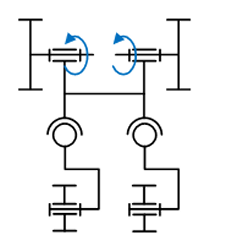
\includegraphics[width=2.5cm]{pictures/chapter2/robot_swd.png} & 
                - Hai bánh chủ động phía trước kéo tải nên khó lật. \newline
                - Khả năng cân bằng tốt \newline
                - Độ ổn định khi chuyển hướng tốt & 
                - Khả năng bám đường không tốt, vào cua ở tốc độ cao dễ bị trượt. \newline
                - Mô hình tính toán phức tạp, khó điều khiển. \\
                \hline
                Robot Usain Bolt 2.0 \newline
                \textit{Phương án 3} \newline
                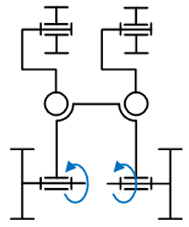
\includegraphics[width=2.5cm]{pictures/chapter2/robot_usain.png} & 
                - Kết cấu 4 bánh giúp tăng khả năng tải. \newline
                - Khả năng vào cua và bám đường tốt. \newline
                - Kết cấu cơ khí đơn giản & 
                - Đảm bảo đồng trục 2 bánh dẫn động. \newline
                - Đảm bảo đồng phẳng giữa các bánh xe. \newline
                - Bị hóc đầu nếu đặt tải lệch về phía sau. \newline
                - Dễ bị lật khi vào cua với tốc độ cao. \newline
                - Mô hình tính toán phức tạp, khó điều khiển. \\
                \hline
                Robot Khepera IV \newline
                \textit{Phương án 4} \newline
                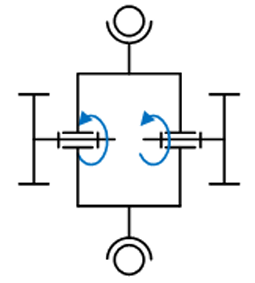
\includegraphics[width=2.5cm]{pictures/chapter2/robot_khepera_IV.png} &
                - Kết cấu 4 bánh đơn giản, mô hình toán đơn giản, dễ điều khiển.\newline 
                - Trọng tâm nằm ngay trục dẫn động giữ kết cấu dễ ổn định. &
                - Khả năng vào cua kém. \newline
                - Đảm bảo đồng trục giữa 2 bánh dẫn động và đồng phẳng giữa các bánh. \newline
                - Hai bánh giữa chịu áp lực lớn vừa chịu tải vừa kéo tải. \\
                \hline
                Robot FireBall \newline
                \textit{Phương án 5} \newline
                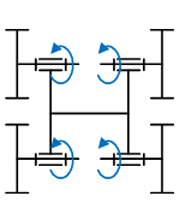
\includegraphics[width=2.5cm]{pictures/chapter2/robot_fireball.png} &
                - Kết cấu cơ khí đơn giản, cân bằng tốt. \newline
                - Tải chia đều cho 4 động cơ -> giảm tải. \newline
                - Điều khiển tùy ý dễ dàng. &
                - Đảm bảo đồng trục cả 2 bánh trước và 2 bánh sau. \newline
                - Đảm bảo đồng phẳng giữa các bánh. \newline
                - Mô hình tính toán phức tạp, khó điều khiển. \\ 
            \end{longtable}
            \hspace*{0.6cm}Qua bảng so sánh trên, ta thấy phương án 3 là phương án tối ưu nhất, đáp ứng được
    \chapter{TÍNH TOÁN, THIẾT KẾ HỆ THỐNG ĐIỆN}
    \section{Thiết kế sơ đồ nguyên lý điện}
        \begin{figure}[H]
            \centering
            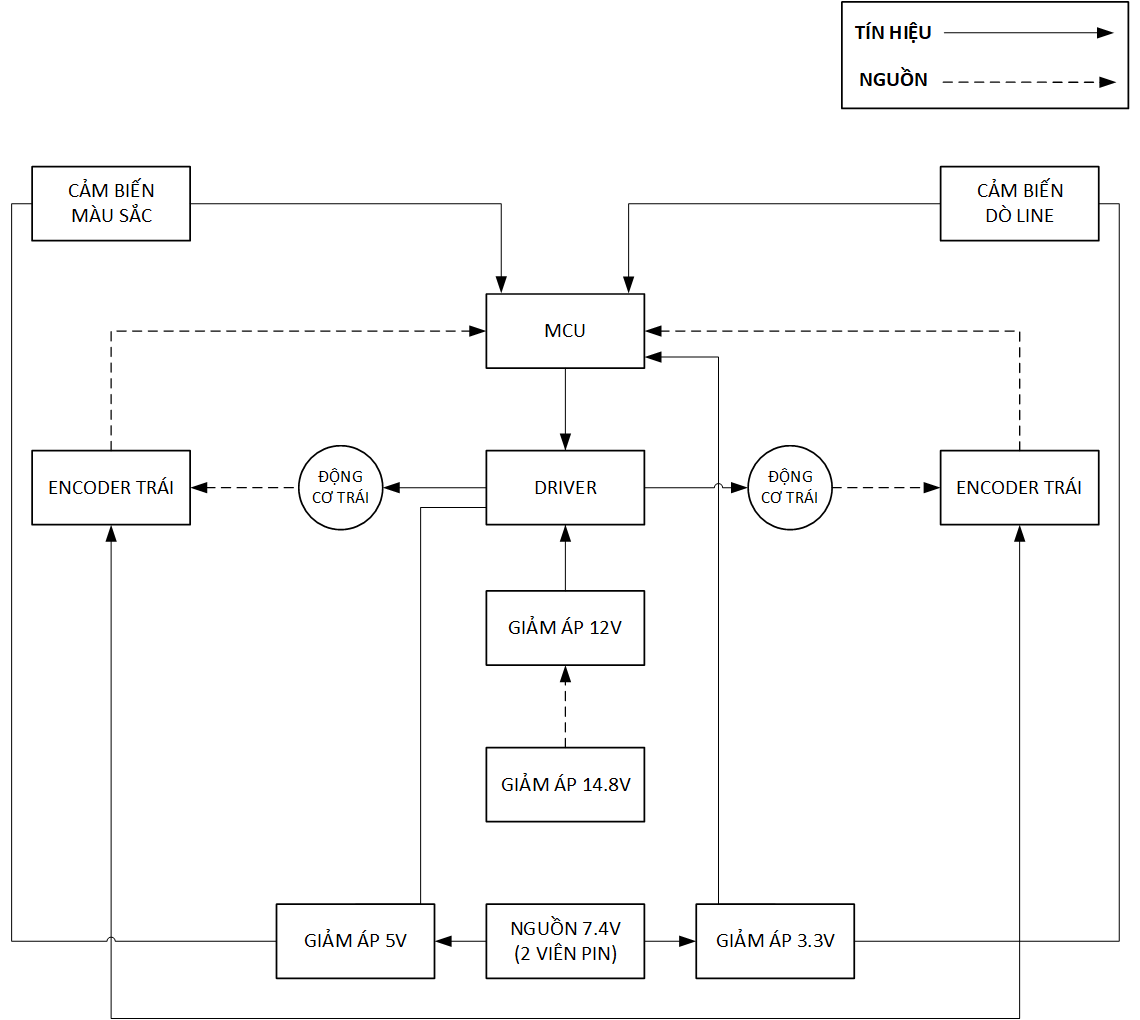
\includegraphics[width=1\textwidth]{pictures/chapter4/c4_p1_ElectricalFlow.png}
            \caption{Sơ đồ nguyên lý điện của hệ thống}
            \label{fig:4-1}
        \end{figure}
    \section{Thiết kế mạch cảm biến}
        \hspace*{0.6cm}Theo tài liệu tham khảo \cite{vishay_tcrt5000_1}, ta có bảng đặc tính kỹ thuật của cảm biến TCRT5000 như sau:
        \begin{table}[H]
            \centering
            \caption{Đặc tính kỹ thuật của cảm biến TCRT5000}
            \label{tab:4-1}
            \begin{tabular}{|c|c|}
                \hline
                \textbf{Thông số} & \textbf{Giá trị} \\
                \hline
                Khoảng cách hoạt động & 0.2 - 15 (mm) \\
                \hline
                Kích thước bao & 10.2 x 5.8 x 7 (mm) \\
                \hline
                Góc phát & $16^{\circ}$ \\
                \hline
                Góc thu & $30^{\circ}$ \\
                \hline
                $I_{C}$ (max) & 100 (mA) \\
                \hline
                $I_{F}$ (max) & 60 (mA) \\
                \hline
            \end{tabular}
        \end{table}
        \subsection{Tính chọn điện trở cho cảm biến dò line}
            \begin{figure}[H]
                \centering
                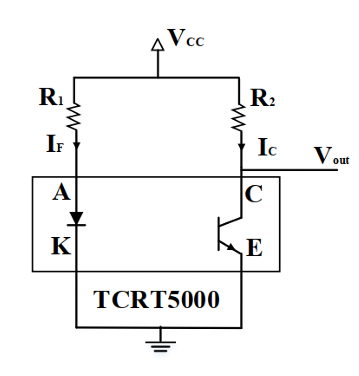
\includegraphics[width=0.3\textwidth]{pictures/chapter4/c4_p2_TCRT5000Schematic.png}
                \caption{Sơ đồ mạch điện TCRT5000}
                \label{fig:4-4}
            \end{figure}
            \hspace*{0.6cm}Dựa vào đường đặc tuyến trên datasheet, ta chọn $V_{F} = 1.1$ (V) và $I_{F} = 10$ (mA).\\
            \begin{figure}[H]
                \centering
                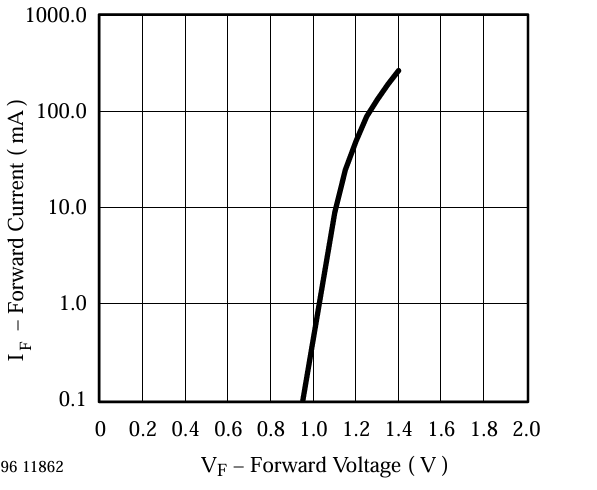
\includegraphics[width=0.5\textwidth]{pictures/chapter4/c4_p3_Voltage&Current.png}
                \caption{Đường đặc tuyến $V_{F}$ và $I_{F}$ của TCRT5000}
                \label{fig:4-5}
            \end{figure}
            Để tính điện trở R1, ta sử dụng công thức:
            \begin{equation}
                R_{1} = \frac{V_{CC} - V_{F}}{I_{F}} = \frac{3.3 - 1.1}{0.01} = 220 \Omega
                \label{eq:4-1}
            \end{equation}
            \hspace*{0.6cm}Chọn điện trở R1 là $220 \Omega$ theo tiêu chuẩn trên thị trường.\\[0.4cm]
            \hspace*{0.6cm}Từ đường đặc tuyến $I_{C} - I_{F}$. Với $I_{F} = 10$ (mA) $\Rightarrow$ $I_{C} \approx 1$ (mA).
            \begin{figure}[H]
                \centering
                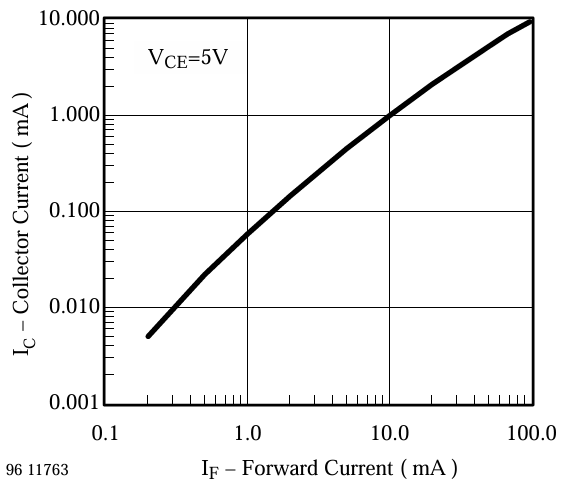
\includegraphics[width=0.5\textwidth]{pictures/chapter4/c4_p4_IC&IF.png}
                \caption{Đường đặc tuyến $I_{C}$ và $I_{F}$ của TCRT5000}
                \label{fig:4-6}
            \end{figure}
            Từ đường đặc tuyến $V_{CE} - I_{C} - I_{F}$, với $I_{C} = 1$ (mA) và $I_{F} = 10$ (mA) $\Rightarrow$ $V_{CE} \approx 1$ (V).\\
            \begin{figure}[H]
                \centering
                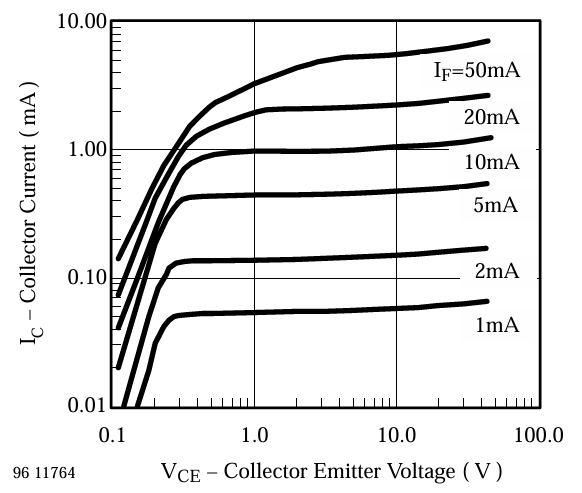
\includegraphics[width=0.5\textwidth]{pictures/chapter4/c4_p5_VCE&IC&IF.png}
                \caption{Đường đặc tuyến $V_{CE}$, $I_{C}$ và $I_{F}$ của TCRT5000}
                \label{fig:4-7}
            \end{figure}
            Từ đó, ta tính điện trở R2:
            \begin{equation}
                R_{2} = \frac{V_{CC} - V_{CE}}{I_{C}} = \frac{3.3 - 1}{0.001} = 2300 \Omega
                \label{eq:4-2}
            \end{equation}
            \hspace*{0.6cm}Chọn điện trở R2 là $2.4 k\Omega$ theo tiêu chuẩn trên thị trường.
        \subsection{Xác định cách đặt cảm biến}
            \hspace*{0.6cm}Có 2 cách đặt cảm biến dò line:
            \begin{itemize}
                \item Trục giữa của bộ phát (S) và thu (E) vuông góc với biên phân cách sáng – tối (Position 1).
                \item Trục giữa của bộ phát (S) và thu (E) song song với biên phân cách sáng – tối (Position 2).
            \end{itemize}
            \begin{figure}[H]
                \centering
                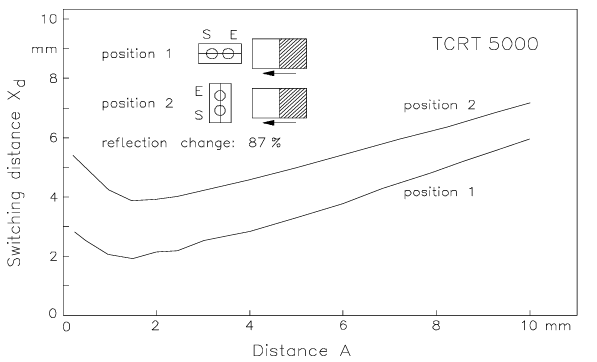
\includegraphics[width=0.8\textwidth]{pictures/chapter4/c4_p6_SensorPosition.png}
                \caption{So sánh độ phân giải của cảm biến khi đặt ở 2 vị trí khác nhau}
                \label{fig:4-8}
            \end{figure}
            \hspace*{0.6cm}Từ hình trên, ta thấy vị trí đặt cảm biến như Position 1 sẽ cho độ phân giải cao hơn so với Position 2. Do đó, ta chọn cách đặt cảm biến ở Position 1.
        \subsection{Xác định khoảng cách giữa cảm biến dò line và sa bàn}
            \hspace*{0.6cm}Theo datasheet, trong khoảng cách từ 0.2 - 15 mm thì cảm biến cho kết quả tốt nhất. Do đó tiến hành đo giá trị ADC từ cảm biến trong khoảng 1 - 15mm trên sa bản và thu được kết quả.
            \begin{table}[H]
                \centering
                \caption{Giá trị ADC từ cảm biến dò line ở các khoảng cách khác nhau}
                \label{tab:4-2}
                \begin{tabular}{|c|c|c|c|}
                    \hline
                    \textbf{h (mm)} & \textbf{Giá trị vùng trắng} & \textbf{Giá trị vùng đen} & \textbf{Chênh lệch} \\
                    \hline
                    1 & 39 & 814 & 775 \\
                    \hline
                    2 & 37 & 798 & 761 \\
                    \hline
                    3 & 37 & 785 & 748 \\
                    \hline
                    4 & 34 & 786 & 752 \\
                    \hline
                    5 & 36 & 793 & 757 \\
                    \hline
                    6 & 37 & 797 & 760 \\
                    \hline
                    7 & 36 & 804 & 768 \\
                    \hline
                    \rowcolor{yellow!50}
                    8 & 38 & 841 & 803 \\
                    \hline
                    \rowcolor{yellow!50}
                    9 & 39 & 856 & 817 \\
                    \hline
                    \rowcolor{yellow!50}
                    10 & 40 & 864 & 824 \\
                    \hline
                    \rowcolor{yellow!50}
                    11 & 41 & 878 & 837 \\
                    \hline
                    \rowcolor{yellow!50}
                    12 & 53 & 894 & 841 \\
                    \hline
                    13 & 134 & 872 & 738 \\
                    \hline
                    14 & 162 & 936 & 774 \\
                    \hline
                    15 & 231 & 896 & 665 \\
                    \hline
                \end{tabular}
            \end{table}
            \begin{figure}[H]
                \centering
                \begin{tikzpicture}
                    \begin{axis}[
                        width=14cm,
                        height=8cm,
                        xlabel={Khoảng cách h (mm)},
                        ylabel={Giá trị ADC},
                        legend pos=north west,
                        grid=major,
                        xmin=0, xmax=16,
                        ymin=0, ymax=1000,
                        mark size=2pt
                    ]
                    
                    % Đường giá trị vùng trắng
                    \addplot[color=blue, mark=o, thick] coordinates {
                        (1,39) (2,37) (3,37) (4,34) (5,36) (6,37) (7,36) 
                        (8,38) (9,39) (10,40) (11,41) (12,53) (13,134) 
                        (14,162) (15,231)
                    };
                    \addlegendentry{Vùng trắng}
                    
                    % Đường giá trị vùng đen
                    \addplot[color=red, mark=square, thick] coordinates {
                        (1,814) (2,798) (3,785) (4,786) (5,793) (6,797) (7,804) 
                        (8,841) (9,856) (10,864) (11,878) (12,894) (13,872) 
                        (14,936) (15,896)
                    };
                    \addlegendentry{Vùng đen}
                    
                    % Highlight vùng tối ưu (8-12mm)
                    \addplot[color=gray, fill=yellow, fill opacity=0.3, draw=none] 
                    coordinates {(8,0) (8,1000) (12,1000) (12,0)} \closedcycle;
                    
                    \end{axis}
                \end{tikzpicture}
                \caption{Đồ thị giá trị ADC theo khoảng cách cảm biến}
                \label{fig:4.9}
            \end{figure}

            % Vẽ đồ thị chênh lệch
            \begin{figure}[H]
                \centering
                \begin{tikzpicture}
                    \begin{axis}[
                        width=14cm,
                        height=8cm,
                        xlabel={Khoảng cách h (mm)},
                        ylabel={Chênh lệch giá trị ADC},
                        grid=major,
                        xmin=0, xmax=16,
                        ymin=600, ymax=900,
                        mark size=2pt
                    ]
                    
                    % Đường chênh lệch
                    \addplot[color=green, mark=triangle, thick] coordinates {
                        (1,775) (2,761) (3,748) (4,752) (5,757) (6,760) (7,768) 
                        (8,803) (9,817) (10,824) (11,837) (12,841) (13,738) 
                        (14,774) (15,665)
                    };
                    
                    % Highlight vùng tối ưu
                    \addplot[color=gray, fill=green, fill opacity=0.2, draw=none] 
                    coordinates {(8,600) (8,900) (12,900) (12,600)} \closedcycle;
                    
                    \end{axis}
                \end{tikzpicture}
                \caption{Đồ thị chênh lệch giá trị ADC theo khoảng cách}
                \label{fig:4.10}
            \end{figure}
            Từ bảng trên ta thấy trong khoảng h từ 8 - 12 mm thì chênh lệch giá trị ADC giữa vùng trắng và vùng đen là lớn nhất và ổn định nhất. Do đó, ta tiếp tục cho cảm biến đi ngang qua đường line với quãng đường 20mm quanh ranh giới trắng và đen trong khoảng h từ 8 - 12 mm để xác định độ cao thích hợp nhất.
            \begin{table}[H]
                \centering
                \caption{Giá trị ADC khi cảm biến đi qua đường line với khoảng cách khác nhau}
                \label{tab:4-3}
                \begin{tabular}{|c|c|c|c|c|c|c|c|c|c|c|c|}
                    \hline
                    \textbf{h} & \textbf{0} & \textbf{1} & \textbf{2} & \textbf{3} & \textbf{4} & \textbf{5} & \textbf{6} & \textbf{7} & \textbf{8} & \textbf{9} & \textbf{10} \\
                    \hline
                    \textbf{8} & 45 & 44 & 54 & 135 & 200 & 285 & 345 & 491 & 623 & 655 & 713 \\
                    \hline
                    \textbf{9} & 43 & 43 & 52 & 130 & 190 & 280 & 340 & 503 & 625 & 662 & 721 \\
                    \hline
                    \textbf{10} & 45 & 43 & 52 & 93 & 195 & 277 & 332 & 505 & 609 & 674 & 739 \\
                    \hline
                    \textbf{11} & 43 & 43 & 50 & 112 & 189 & 263 & 349 & 482 & 615 & 663 & 698 \\
                    \hline
                    \textbf{12} & 41 & 40 & 44 & 90 & 167 & 233 & 313 & 473 & 591 & 639 & 679 \\
                    \hline
                \end{tabular}
                \begin{tabular}{|c|c|c|c|c|c|c|c|c|c|c|}
                    \hline
                    \textbf{h} & \textbf{11} & \textbf{12} & \textbf{13} & \textbf{14} & \textbf{15} & \textbf{16} & \textbf{17} & \textbf{18} & \textbf{19} & \textbf{20} \\
                    \hline
                    \textbf{8} & 790 & 819 & 850 & 855 & 865 & 870 & 855 & 878 & 875 & 877 \\
                    \hline
                    \textbf{9} & 785 & 823 & 845 & 850 & 860 & 865 & 850 & 873 & 870 & 872 \\
                    \hline
                    \textbf{10} & 794 & 836 & 848 & 853 & 863 & 863 & 862 & 862 & 860 & 863 \\
                    \hline
                    \textbf{11} & 787 & 825 & 857 & 861 & 867 & 873 & 877 & 877 & 875 & 876 \\
                    \hline
                    \textbf{12} & 765 & 803 & 825 & 836 & 844 & 849 & 849 & 852 & 857 & 855 \\
                    \hline
                \end{tabular}
            \end{table}

            \begin{figure}[H]
                \centering
                \begin{tikzpicture}
                    \begin{axis}[
                        width=16cm,
                        height=10cm,
                        xlabel={Vị trí cảm biến (mm)},
                        ylabel={Giá trị ADC},
                        legend pos=north west,
                        grid=major,
                        xmin=-1, xmax=21,
                        ymin=0, ymax=1000,
                        mark size=1.5pt,
                        legend style={font=\small}
                    ]
                    
                    % h = 8mm (màu xanh dương)
                    \addplot[color=blue, mark=none, thick, smooth] coordinates {
                        (0,45) (1,44) (2,54) (3,135) (4,200) (5,285) (6,345) (7,491) (8,623) (9,655) 
                        (10,713) (11,790) (12,819) (13,850) (14,855) (15,865) (16,870) (17,855) (18,878) (19,875) (20,877)
                    };
                    \addlegendentry{8}
                    
                    % h = 9mm (màu cam)
                    \addplot[color=orange, mark=none, thick, smooth] coordinates {
                        (0,43) (1,43) (2,52) (3,130) (4,190) (5,280) (6,340) (7,503) (8,625) (9,662) 
                        (10,721) (11,785) (12,823) (13,845) (14,850) (15,860) (16,865) (17,850) (18,873) (19,870) (20,872)
                    };
                    \addlegendentry{9}
                    
                    % h = 10mm (màu đỏ - highlight)
                    \addplot[color=red, mark=none, thick, smooth] coordinates {
                        (0,45) (1,43) (2,52) (3,93) (4,195) (5,277) (6,332) (7,505) (8,609) (9,674) 
                        (10,739) (11,794) (12,836) (13,848) (14,853) (15,863) (16,863) (17,862) (18,862) (19,860) (20,863)
                    };
                    \addlegendentry{10}
                    
                    % h = 11mm (màu vàng)
                    \addplot[color=yellow!80!black, mark=none, thick, smooth] coordinates {
                        (0,43) (1,43) (2,50) (3,112) (4,189) (5,263) (6,349) (7,482) (8,615) (9,663) 
                        (10,698) (11,787) (12,825) (13,857) (14,861) (15,867) (16,873) (17,877) (18,877) (19,875) (20,876)
                    };
                    \addlegendentry{11}
                    
                    % h = 12mm (màu xanh nhạt)
                    \addplot[color=cyan, mark=none, thick, smooth] coordinates {
                        (0,41) (1,40) (2,44) (3,79) (4,167) (5,233) (6,313) (7,473) (8,591) (9,639) 
                        (10,679) (11,765) (12,803) (13,825) (14,836) (15,844) (16,849) (17,849) (18,852) (19,857) (20,855)
                    };
                    \addlegendentry{12}
                    
                    % Đánh dấu vị trí chuyển line tại x = 10
                    \addplot[color=black, mark=none, thick, dashed] coordinates {(10,0) (10,1000)};
                    
                    % Thêm text đánh dấu
                    \node[anchor=south] at (axis cs:10,900) {\textbf{Chuyển line}};
                    \node[anchor=south] at (axis cs:10,850) {\textbf{(Vị trí 10)}};
                    
                    % Đánh dấu vùng trước và sau line
                    \node[anchor=center] at (axis cs:5,600) {\textbf{Vùng trắng}};
                    \node[anchor=center] at (axis cs:15,600) {\textbf{Vùng đen}};
                    
                    \end{axis}
                \end{tikzpicture}
                \caption{Biểu đồ giá trị ADC khi cảm biến đi qua đường line}
                \label{fig:4-11}
            \end{figure}
            Từ bảng và đồ thị trên, ta thấy tại h = 10mm, cảm biến cho kết quả chuyển tiếp rõ ràng và nhanh nhất giữa nền trắng và nền đen. Do đó, ta chọn khoảng cách từ cảm biến dò line đến sa bàn là 10mm.

        \subsection{Xác định khoảng cách giữa các cảm biến}
            \begin{figure}[H]
                \centering
                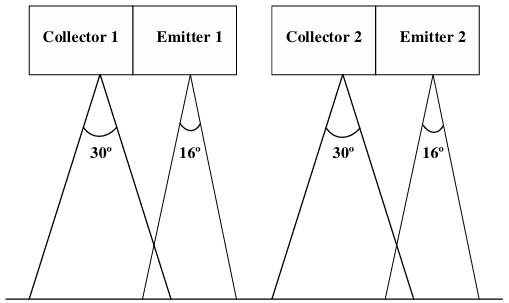
\includegraphics[width=0.7\textwidth]{pictures/chapter4/c4_p7_DistanceCollectorEmitter1.png}
                \label{fig:4-12}
                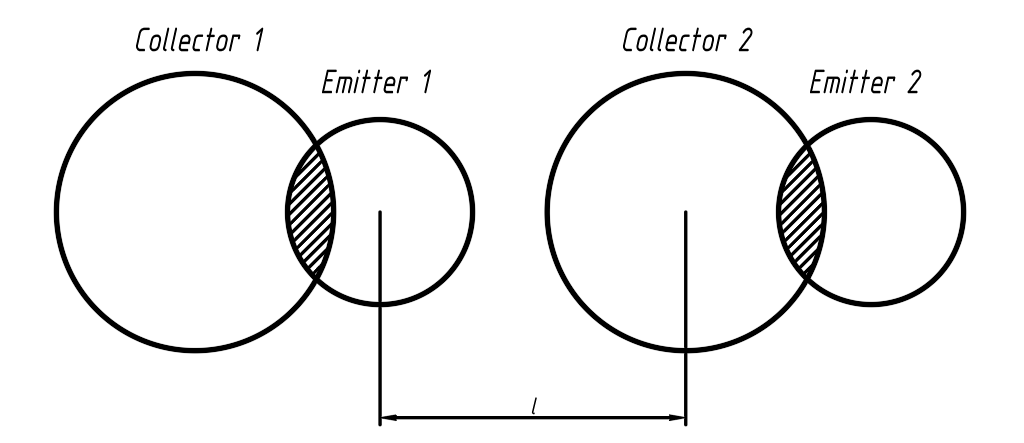
\includegraphics[width=0.8\textwidth]{pictures/chapter4/c4_p8_DistanceCollectorEmitter2.png}
                \caption{Khoảng cách giữa các vùng thu và vùng phát}
                \label{fig:4-13}
                \end{figure}
            \hspace*{0.6cm}Với h = 10mm, ta tính khoảng cách giữa vùng phát và vùng thu liền kề nhau tối thiểu để không bị giao thoa là:
            \begin{align}
                l_{min} &= (r + R) \label{eq:4-3} \\
                        &= (h +0.7) \times \tan{8^{\circ}} + (h + 0.7) \times \tan{15^{\circ}} \nonumber \\
                        &= (10 + 0.7) \times \tan{8^{\circ}} + (10 + 0.7) \times \tan{15^{\circ}} \nonumber \\
                        &= 4.4 \text{ (mm)} \nonumber
            \end{align}
            \hspace*{0.6cm}Khoảng cách tối thiểu giữa 2 cảm biến là:
            \begin{align}
                d_{min} = l_{min} + d = 4.4 + 3.8 = 8.2 \text{ (mm)}
                \label{eq:4-4}
            \end{align}
            \hspace*{0.6cm}Dựa vào datasheet, ta có chiều dài của cảm biến TCRT5000 là 10.2 mm (bố trí nằm ngang). Do đó, với độ cao $h = 10$ mm thì chắc chắn hai cảm biến liền kề không ảnh hưởng nhau.\\[0.4cm]
            \begin{figure}[H]
                \centering
                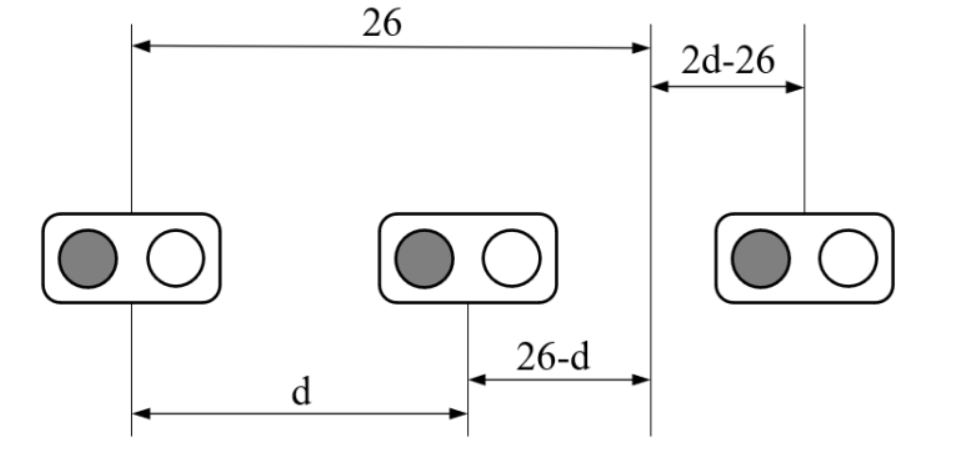
\includegraphics[width=0.8\textwidth]{pictures/chapter4/c4_p9_SensorDistance.png}
                \caption{Khoảng cách giữa các cảm biến dò line}
                \label{fig:4-14}
            \end{figure}
            Do line có bề rộng là 26mm nên tối đa có 3 cảm biến có vùng phát hiện nằm trong line. Bên cạnh đó, khi hoạt động sẽ có trường hợp cảm biến rơi vào vùng bất định thì giá trị analog trả về từ cảm biến sẽ như nhau. Do đó, không thể tính toán sai số để xác định được vị trí cảm biến so với đường tâm line. \\
            \hspace*{0.6cm}Ta xét các trường hợp:
            \begin{itemize}
                \item Trường hợp 1: Khi di chuyển sang phải trong khoảng 26 - d thì có 2 led nằm trong line nên thuđược giá trị analog là như nhau dẫn đến cảm biến rơi vào vùng bất định. 
                \item Trường hợp 2: Khi di chuyển sang trái trong khoảng 2d - 26 thì chỉ có 1 led nằm trên đường line và cũng rơi vào vùng bất định. 
            \end{itemize}
            \hspace*{0.6cm}Do đó để hạn chế việc cảm biến rơi vào vùng bất định thì lựa chọn khoảng cách $d$ sao cho $f_1 = 26 - d$ và $f_2 = 2d - 26$ là nhỏ nhất. \\
            \hspace*{0.6cm}Do $f_1$ là hàm đơn điệu giảm, $f_2$ là hàm đơn điệu tăng nên để $f_1$ và $f_2$ là nhỏ nhất thì ta chọn $f_1 = f_2$. Từ đó ta có:
            \begin{align}
                f_1 &= f_2 \label{eq:4-5}\\
                \Rightarrow 26 - d &= 2d - 26 \nonumber \\
                \Rightarrow d &= 17.33 \text{ (mm)} \nonumber
            \end{align}
        \subsection{Thiết kế sơ đồ nguyên lý mạch cảm biến}
            \hspace*{0.6cm}Dựa vào các tính toán trên, ta thiết kế sơ đồ nguyên lý mạch cảm biến như sau:
            \begin{itemize}
                \item Sử dụng 5 cảm biến TCRT5000 được bố trí nằm ngang vuông góc theo đường line.
                \item Khoảng cách từ cảm biến đến sa bàn là 10mm.
                \item Khoảng cách giữa các cảm biến là 17mm.
                \item Điện trở R1 là 220$\Omega$ và R2 là 2.4k$\Omega$.
            \end{itemize}
            \begin{figure}[H]
                \centering
                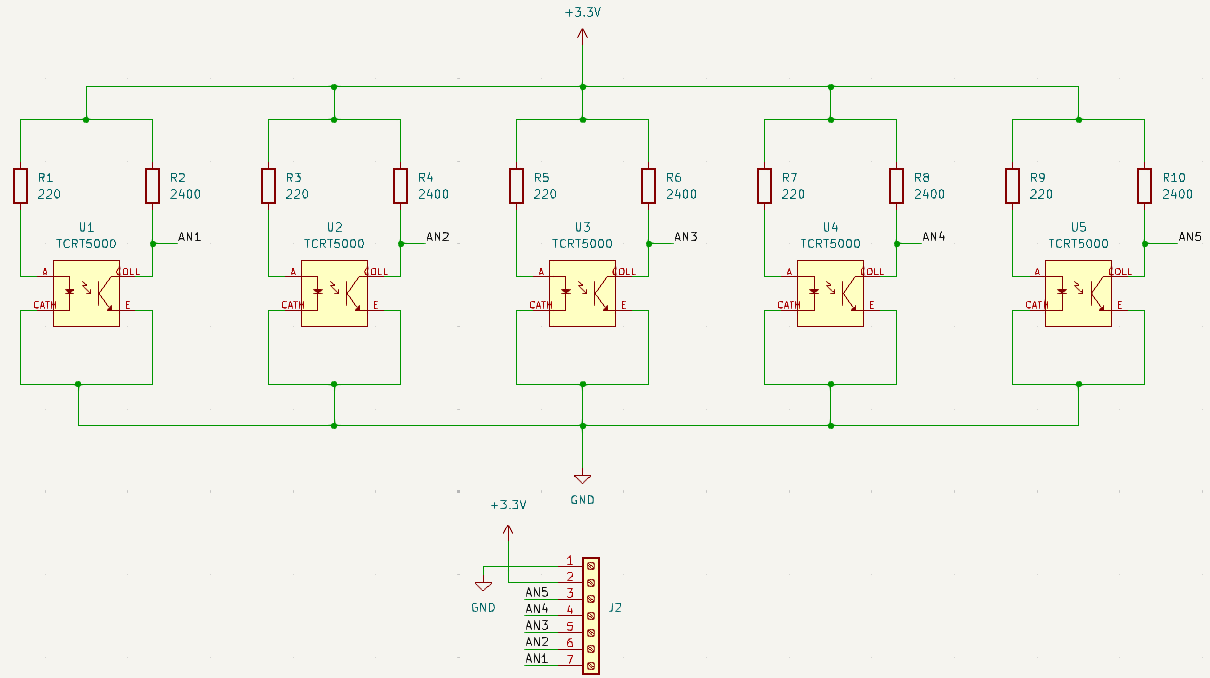
\includegraphics[width=1\textwidth]{pictures/chapter4/c4_p10_SensorSchematic.png}
                \caption{Sơ đồ nguyên lý mạch cảm biến dò line}
                \label{fig:4-15}
            \end{figure}
        \subsection{Thiết kế PCB mạch cảm biến}

            \hspace*{0.6cm}Dựa vào sơ đồ nguyên lý mạch cảm biến, ta tiến hành thiết kế PCB cho mạch cảm biến dò line. Sơ đồ thiết kế PCB được trình bày như hình \ref{fig:4-16}.

            \begin{figure}[H]
                \centering
                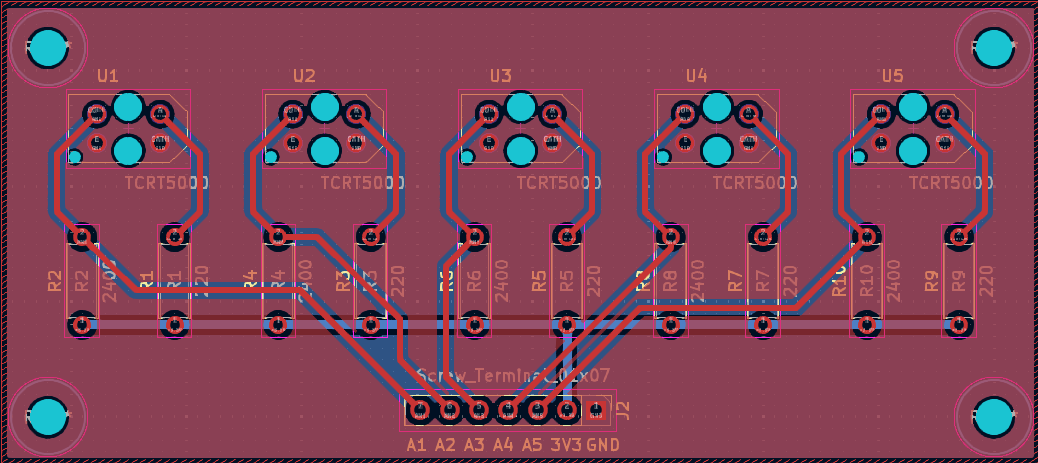
\includegraphics[width=1\textwidth]{pictures/chapter4/c4_p11_SensorPCB.png}
                \caption{Sơ đồ thiết kế PCB mạch cảm biến dò line}
                \label{fig:4-16}
            \end{figure}
        \subsection{Calib và tuyến tính hóa cảm biến}
            \hspace*{0.6cm}Mỗi cảm biến dò line sẽ trả về tín hiệu analog khác nhau trong cùng điều kiện. Do đó, việc calib cảm biến là vô cùng cần thiết. Lựa chọn phương pháp calib bằng công thức:
            \begin{align}
                y_i = y_{min} + \frac{(y_{max} - y_{min})(x_{ij} - x_{min, i})}{x_{max, i} - x_{min, i}} 
                \label{eq:4-6}
            \end{align}
            \hspace*{0.6cm}Trong đó:
            \begin{itemize}
                \item $x_{max,i}$ và $x_{min,i}$: giá trị analog lớn nhất và nhỏ nhất của cảm biến thứ $i$.
                \item $y_{max}$ và $y_{min}$: giá trị analog lớn nhất và nhỏ nhất mà ta mong muốn cho tất cả cảm biến.
                \item $x_{ij}$: giá trị analog đọc về từ cảm biến thứ $i$.
                \item $y_{i0}$: giá trị analog đọc về sau khi đã calib của cảm biến thứ $i$.
            \end{itemize}
            \begin{table}[H]
                \centering
                \caption{Bảng giá trị analog của cảm biến trước khi calib ở độ cao h = 10mm}
                \label{tab:4-4}
                \begin{tabular}{|c|c|c|}
                    \hline
                    \textbf{Cảm biến} & $\mathbf{x_{max,i}}$ & $\mathbf{x_{min,i}}$  \\
                    \hline
                    Cảm biến 1 & 870 & 54  \\
                    \hline
                    Cảm biến 2 & 805 & 51  \\
                    \hline
                    Cảm biến 3 & 872 & 73  \\
                    \hline
                    Cảm biến 4 & 855 & 65  \\
                    \hline
                    Cảm biến 5 & 863 & 88  \\
                    \hline
                \end{tabular}
            \end{table}
            \hspace*{0.6cm}Dựa vào giá trị trung bình, ta có được giá trị mong muốn: $y_{max} = 853$ và $y_{min} = 66$.\\
            \hspace*{0.6cm}Từ đó ta có công thức calib cho từng cảm biến:
            \begin{itemize}
                \item Cảm biến 1:
                \begin{align*}
                    y_1 = 66 + \frac{(853 - 66)(x_{1j} - 54)}{870 - 54} = 66 + 0.88(x_{1j} - 54)
                \end{align*}
                \item Cảm biến 2:
                \begin{align*}
                    y_2 = 66 + \frac{(853 - 66)(x_{2j} - 51)}{805 - 51} = 66 + 0.95(x_{2j} - 51)
                \end{align*}
                \item Cảm biến 3:
                \begin{align*}
                    y_3 = 66 + \frac{(853 - 66)(x_{3j} - 73)}{872 - 73} = 66 + 0.88(x_{3j} - 73)
                \end{align*}
                \item Cảm biến 4:
                \begin{align*}
                    y_4 = 66 + \frac{(853 - 66)(x_{4j} - 65)}{855 - 65} = 66 + 0.91(x_{4j} - 65)
                \end{align*}
                \item Cảm biến 5:
                \begin{align*}
                    y_5 = 66 + \frac{(853 - 66)(x_{5j} - 88)}{863 - 88} = 66 + 0.89(x_{5j} - 88)
                \end{align*}
            \end{itemize}
        \subsection{Tìm giá trị sai số theo phương pháp trung bình trọng số}
            \hspace*{0.6cm}Giá sử tọa độ của 5 cảm biến lần lượt là $x_1, x_2, x_3, x_4, x_5$ so với tâm đường line và các giá trị analog tương ứng là $y_1, y_2, y_3, y_4, y_5$. Từ đó, ta tìm được vị trí xe so với tâm đường line theo công thức sau:
            \begin{equation}
                X = L_{cb} \times \frac{\sum_{i=1}^{5} x_i y_i}{\sum_{i=1}^{5} y_i} = 17 \times \frac{2(y_5 - y_1) + (y_4 - y_2)}{y_1 + y_2 + y_3 + y_4 + y_5}
                \label{eq:4-7}
            \end{equation}

            Tiến hành thực nghiệm đọc tín hiệu cảm biến với bước nhảy 1 mm, giới hạn từ $-30$ mm tới $30$ mm so với tâm đường line bằng máy in 3D theo quy trình sau:
            \begin{itemize}
                \item Bước 1: Tiến hành gá cụm cảm biến lên cụm in của máy in 3D.
                \item Bước 2: Di chuyển trục z về vị trí home là vị trí cách mặt in đúng bằng khoảng cách từ cảm biến đến line theo tính toán (10 mm).
                \item Bước 3: Dịch chỉnh trục x sao cho cụm cảm biến có cảm biến giữa nằm đúng vị trí tâm line là vị trí mà giá trị cảm biến giữa đọc về lớn nhất.
                \item Bước 4: Di chuyển cụm in sang trái 30 mm và sang phải 30 mm để tiến hành đọc giá trị analog của từng cảm biến.
            \end{itemize}
            \begin{figure}[H]
                \centering
                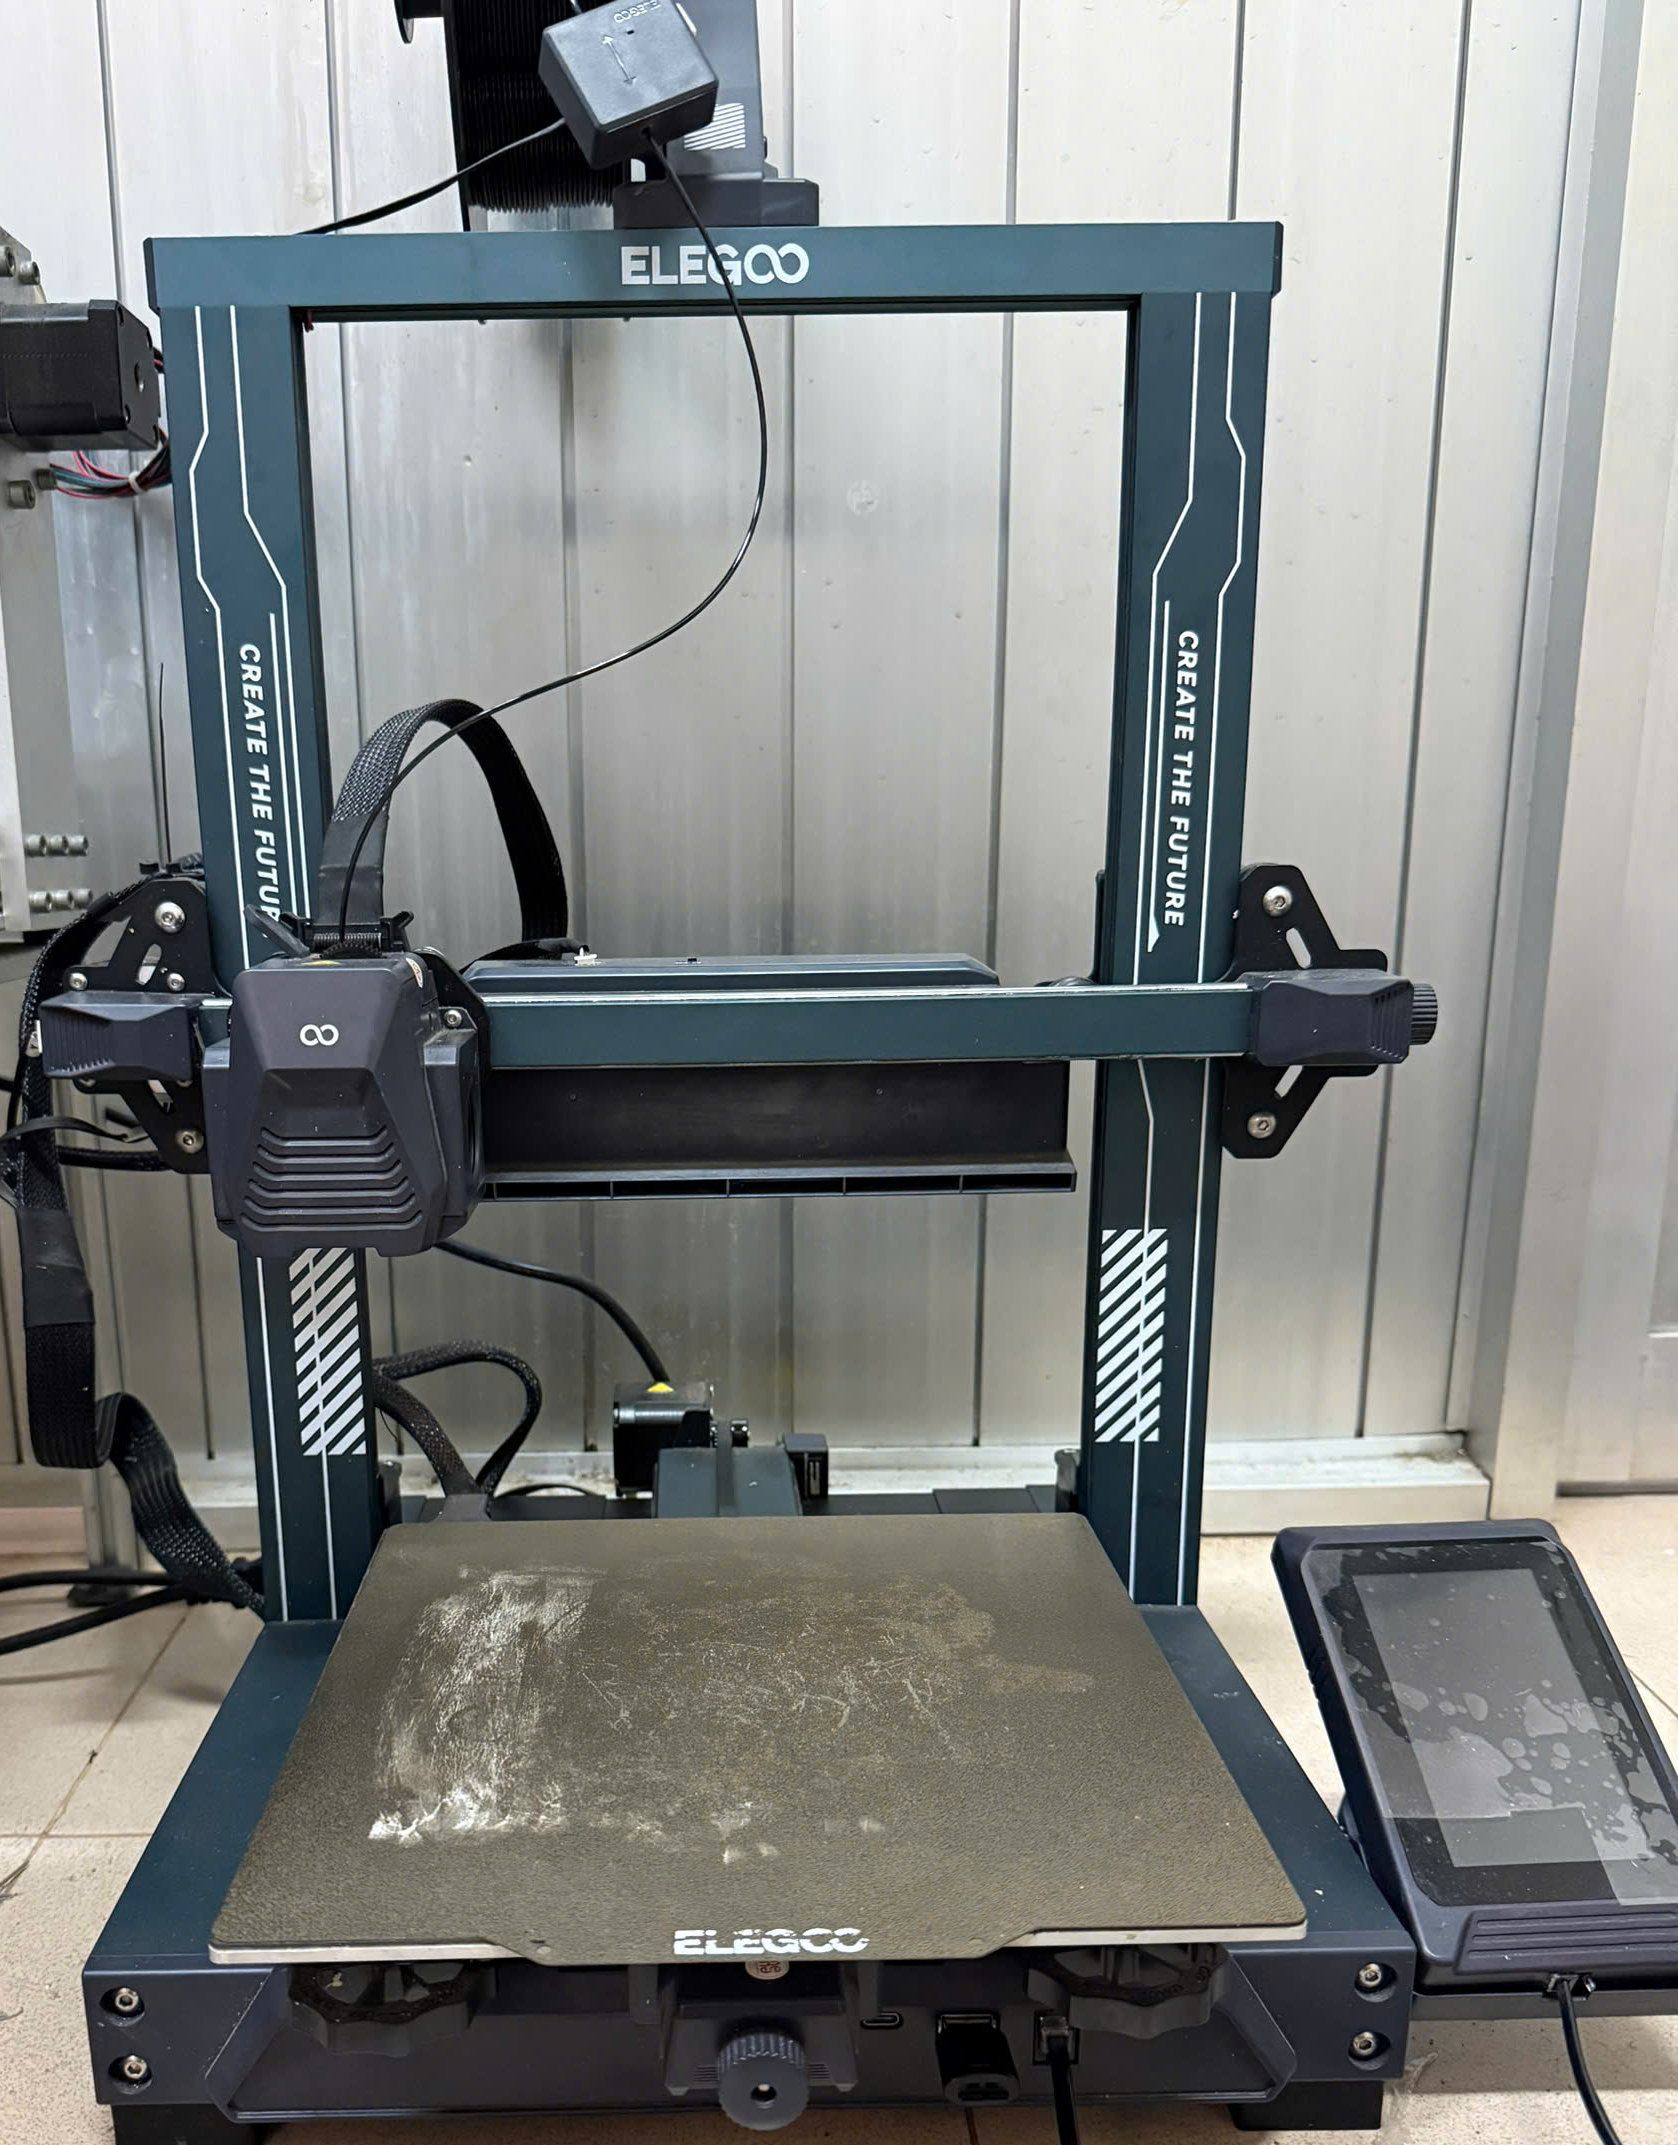
\includegraphics[width=0.6\textwidth]{pictures/chapter4/c4_p16_3DPrinter.png}
                \caption{Máy in 3D dùng để hiệu chuẩn cảm biến dò line}
                \label{fig:4-17}
            \end{figure}
        
            \begin{longtable}{|c|c|c|}
                \caption{Bảng tính toán giá trị sai số giữa vị trí trên thực tế và vị trí tính toán}
                \label{tab:4-5} \\
                \hline
                \textbf{Vị trí (mm)} & \textbf{Giá trị tính toán (mm)} & \textbf{Sai số (mm)} \\
                \hline
                \endfirsthead
                
                \hline
                \textbf{Vị trí (mm)}  & \textbf{Giá trị tính toán (mm)} & \textbf{Sai số (mm)} \\
                \hline
                \endhead
                0 & 0.271428571 & -0.271428571 \\
                \hline
                1 & 0.495008319 & 0.504991681 \\
                \hline
                2 & 2.248142645 & -0.248142645 \\
                \hline
                3 & 4.205958549 & -1.205958549 \\
                \hline
                4 & 5.70234688 & -1.70234688 \\
                \hline
                5 & 6.675065617 & -1.675065617 \\
                \hline
                6 & 7.134005038 & -1.134005038 \\
                \hline
                7 & 7.347029703 & -0.347029703 \\
                \hline
                8 & 7.440652819 & 0.559347181 \\
                \hline
                9 & 7.506713078 & 1.493286922 \\
                \hline
                10 & 7.686354379 & 2.313645621 \\
                \hline
                11 & 8.204347826 & 2.795652174 \\
                \hline
                12 & 9.220866382 & 2.779133618 \\
                \hline
                13 & 10.71843972 & 2.28156028 \\
                \hline
                14 & 12.5566584 & 1.4433416 \\
                \hline
                15 & 12.94961571 & 2.05038429 \\
                \hline
                16 & 13.04991394 & 2.95008606 \\
                \hline
                17 & 13.21570319 & 3.78429681 \\
                \hline
                18 & 14.01160862 & 3.98839138 \\
                \hline
                19 & 16.23355506 & 2.76644494 \\
                \hline
                20 & 18.4286645 & 1.5713355 \\
                \hline
                21 & 20.32566168 & 0.67433832 \\
                \hline
                22 & 21.45665962 & 0.54334038 \\
                \hline
                23 & 22.02743902 & 0.97256098 \\
                \hline
                24 & 22.18875502 & 1.81124498 \\
                \hline
                25 & 22.2288008 & 2.7711992 \\
                \hline
                26 & 22.25314545 & 3.74685455 \\
                \hline
                27 & 22.29408767 & 4.70591233 \\
                \hline
                28 & 22.59401709 & 5.40598291 \\
                \hline
                29 & 23.23741007 & 5.76258993 \\
                \hline
                30 & 24.31478873 & 5.68521127 \\
                \hline
                -30 & -22.63765643 & -7.36234357 \\
                \hline
                -29 & -22.14532148 & -6.85467852 \\
                \hline
                -28 & -21.89844922 & -6.10155078 \\
                \hline
                -27 & -21.79960513 & -5.20039487 \\
                \hline
                -26 & -21.70588235 & -4.29411765 \\
                \hline
                -25 & -21.54179104 & -3.45820896 \\
                \hline
                -24 & -21.11036961 & -2.88963039 \\
                \hline
                -23 & -20.09944751 & -2.90055249 \\
                \hline
                -22 & -18.35491905 & -3.64508095 \\
                \hline
                -21 & -15.75849602 & -5.24150398 \\
                \hline
                -20 & -12.98336106 & -7.01663894 \\
                \hline
                -19 & -12.43197279 & -6.56802721 \\
                \hline
                -18 & -12.26729291 & -5.73270709 \\
                \hline
                -17 & -11.77140482 & -5.22859518 \\
                \hline
                -16 & -10.55522388 & -5.44477612 \\
                \hline
                -15 & -9.357284113 & -5.642715887 \\
                \hline
                -14 & -8.419335706 & -5.580664294 \\
                \hline
                -13 & -7.701092896 & -5.298907104 \\
                \hline
                -12 & -7.182608696 & -4.817391304 \\
                \hline
                -11 & -6.949152542 & -4.050847458 \\
                \hline
                -10 & -6.865708622 & -3.134291378 \\
                \hline
                -9 & -6.833746898 & -2.166253102 \\
                \hline
                -8 & -6.766169154 & -1.233830846 \\
                \hline
                -7 & -6.607287449 & -0.392712551 \\
                \hline
                -6 & -5.884615385 & -0.115384615 \\
                \hline
                -5 & -4.360049322 & -0.639950678 \\
                \hline
                -4 & -1.420972644 & -2.579027356 \\
                \hline
                -3 & 0.014119601 & 3.014119601 \\
                \hline
                -2 & 0.127926421 & 2.127926421 \\
                \hline
                -1 & 0.171428571 & 1.171428571 \\
                \hline        
            \end{longtable}
            \hspace*{0.6cm}Dựa vào số liệu trên, ta thực hiện xấp xỉ tuyến tính giá trị tính toán theo vị trí, thu được phương trình tính xấp xỉ vị trí:
            \begin{align}
                y = 0.8136x - 1.0349
                \label{eq:4-8}
            \end{align}
            Trong đó:
            \begin{itemize}
                \item $y$: giá trị trung bình trọng số (mm).
                \item $x$: vị trí tính toán (mm).
            \end{itemize}
            \begin{figure}[H]
                \centering
                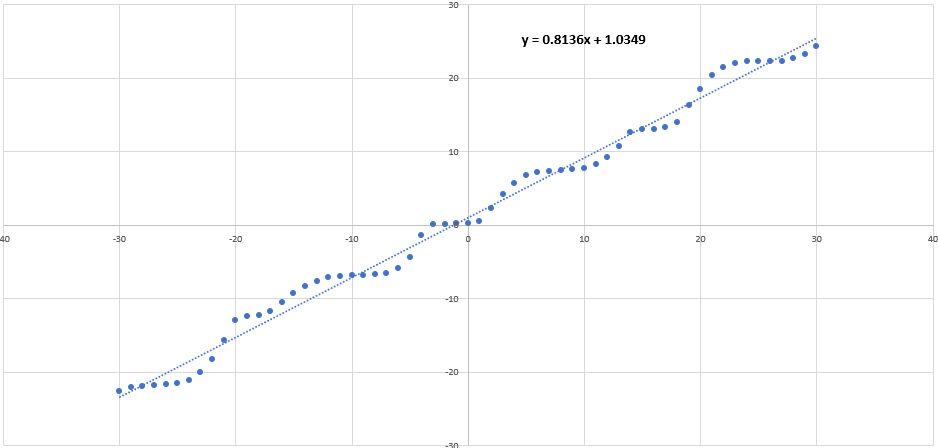
\includegraphics[width=1\textwidth]{pictures/chapter4/c4_p12_LinearRegression.png}
                \caption{Biểu đồ xấp xỉ tuyến tính giá trị tính toán theo vị trí}
                \label{fig:4-8}
            \end{figure}
            \hspace*{0.6cm}Từ bảng số liệu trên, ta có sai số cảm biến lớn nhất đo được là: $e_{max} = 5.8$ mm. \\
    \section{Thiết kế mạch điều khiển} 
        \subsection{Thiết kế mạch nguồn}
            \subsubsection{Nguồn điều khiển}
                \begin{itemize}
                    \item Nguồn điều khiển cần cung cấp cho:
                    \begin{itemize}
                        \item Vi điều khiển STM32F103C8T6: 3.3V
                        \item Mạch cảm biến dò line: 3.3V
                        \item Driver TB6612FNG: 5V
                        \item Cảm biến màu sắc TCS347254: 3.3V
                        \item 2 Encoder: 3.3V
                    \end{itemize}
                    \item Công suất mạch cảm biến:
                    \begin{itemize}
                        \item Công suất tiêu thụ của 5 điện trở $R = 220 \Omega$ trong mạch. \\
                        \begin{align}
                            P_{R1} = 5 \times I_{F}^2 \times R_1 = 5 \times (10.10^{-3})^2 \times 220 = 110 \text{ (mW)}
                        \end{align}
                        \item Công suất tiêu thụ của 5 điện trở $R = 2.4 k\Omega$ trong mạch. \\
                        \begin{align}
                            P_{R2} = 5 \times I_{C}^2 \times R_2 = 5 \times (10^{-3})^2 \times 2400 = 12 \text{ (mW)}
                        \end{align}
                        \item Công suất tiêu thụ của 5 cảm biến TCRT5000 trong mạch. \\
                        \begin{align}
                            P_{TCRT} = 5 \times 200.10^{-3} = 1000 \text{ (mW)}
                        \end{align}
                        Vậy công suất tiêu thụ trên toàn mạch cảm biến:
                        \begin{align}
                            P_{sensor} = P_{R1} + P_{R2} + P_{TCRT} = 110 + 12 + 1000 = 1122 \text{ (mW)}
                        \end{align}
                    \end{itemize}
                    \item Công suất tiêu thụ trên mạch điều khiển:
                    \begin{itemize}
                        \item Công suất tiêu thụ của vi điều khiển STM32F103C8T6 là 363 (mW) và mỗi chân IO sẽ cần 25 (mA) cho dòng điều khiển, vậy tổng công suất:
                        \begin{align}
                            P_{MCU} = 363 + 19 \times 25 \times 3.3 = 1930.5 \text{ (mW)}
                        \end{align}
                        \item Công suất tiêu thụ encoder:
                        \begin{align}
                            P_{encoder} = 2 \times 60 = 120 \text{ (mW)}
                        \end{align}
                        \item Theo datasheet (LM2596 design datasheet) công thức tính xấp xỉ công suất tiêu thụ mạch giảm áp IC LM2596.
                        \begin{align}
                            P_b = (V_{in} \times I_Q) + d \times I_{load} \times V_{sat}
                        \end{align}

                        Trong đó:
                        \begin{itemize}
                            \item $d = \dfrac{V_{out}}{V_{in}}$ \text{duty cycle của mạch giảm áp} \\
                            \item $I_Q = 10 \text{ (mA)}$ \text{tra trong datasheet} \\
                            \item $V_{sat} = 1.4 \text{ (V)}$ \text{tra trong datasheet} \\
                            \item $V_{in}, V_{out}$ \text{điện áp tối thiểu cấp vào, điện áp đầu ra} \\
                            \item $I_{load}$ \text{dòng điện tiêu thụ tải}
                        \end{itemize}

                        Công suất tiêu thụ IC LM2596 5V:
                        \begin{align*}
                            P_{D5} &= (7.4 \times 10 \times 10^{-3}) + \frac{7.4}{5} \times 1.2 \times 1.4 \nonumber = 2560 \text{ (mW)}
                        \end{align*}

                        Công suất tiêu thụ IC LM2596 3.3V:
                        \begin{align*}
                            P_{D3.3} &= (7.4 \times 10 \times 10^{-3}) + \frac{7.4}{3.3} \times (25.10^{-3} \times 19) \times 1.4 \nonumber = 1565 \text{ (mW)}
                        \end{align*}
                        \item Công suất tiêu thụ trên mạch điều khiển:
                        \begin{align}
                            P_{control} &= P_{MCU} + P_{encoder} + P_{D5} + P_{D3.3} \\
                            &= 1930.5 + 120 + 2560 + 1565 = 6175.5 \text{ (mW)}
                        \end{align}
                        \item Công suất tiêu thụ trên mạch tổng:
                        \begin{align}
                            P_{total} &= P_{sensor} + P_{control} \\
                            &= 1122 + 6175.5 = 7297.5 \text{ (mW)}
                        \end{align}
                        \item Dung lượng pin tối thiểu:
                        \begin{align}
                            Q = It = \dfrac{P_{total} \times t}{V} = \dfrac{7297.5 \times 1}{7.4} = 986.15 \text{ (mAh)}
                        \end{align}
                    \end{itemize}
                    \hspace{0.6cm}Với dung lượng pin ta chọn pin 18650 loại 1200 mAh số lượng 2 vì khi dung lượng pin giảm thì điện áp pin giảm nên để đảm bảo nguồn cấp tối thiểu 5V nên chọn số lượng pin là 2.
                \end{itemize}
            \subsubsection{Nguồn động lực}
                \begin{table}[H]
                    \centering
                    \caption{Bảng thông số động cơ JGB37-520}
                    \label{tab:4-5}
                    \begin{tabular}{|c|c|c|c|}
                        \hline
                        \textbf{Thông số} & \textbf{Giá trị} & \textbf{Thông số} & \textbf{Giá trị} \\
                        \hline
                        Loại động cơ & JGB37-520 & Tỉ số truyền & 30:1 \\
                        \hline
                        Dòng không tải & 120 (mA) & Dòng chịu đựng tối đa khi có tải & 1 (A) \\
                        \hline
                        Tốc độ không tải & 333 (rpm) & Tốc độ chịu đựng khi có tải & 250 (rpm) \\
                        \hline
                        Mô men xoắn định mức & 3.5 (kg.cm) & Mô men xoắn tối đa & 5 (kg.cm) \\
                        \hline
                        Chiều dài hộp số L & 22 (mm) & Số xung Encoder mỗi kênh & 330 xung \\
                        \hline
                    \end{tabular}
                \end{table}
                \begin{itemize}
                    \item Công suất của động cơ
                    \begin{align}
                       P_{motor} = T_{max} \times \omega_{max} = 5 \times 0.098 \times \frac{250 \times 2\pi}{60} = 12830 \text{ (mW)}
                    \end{align}
                    \item Công suất tiêu thụ của driver TB6612FNG: \\
                    Ở chế độ điều khiển động cơ với dòng tối đa $I_{max} = 1.2$ (A) và điện áp cung cấp $V_{supply} = 5$ (V), công suất tiêu thụ của driver:
                    \begin{align}
                        P_{Driver} = I_{max} \times V_{supply} = 1.2 \times 5 = 6000 \text{ (mW)}
                    \end{align}
                    \item Công suất của LM2596-12:
                    \begin{align}
                        P_{D12} = (14.8 \times 10 \times 10^{-3}) + \frac{14.8}{12} \times 1.2 \times 1.4 = 2200 \text{ (mW)}
                    \end{align}
                    \item Tổng công suất động lực:
                    \begin{align}
                        P_{dynamic} = 2 \times P_{motor} + P_{Driver} + P_{D12} = 2 \times 12830 + 6000 + 2200 = 33860 \text{ (mW)}
                    \end{align}
                    \item Dung lượng pin tối thiểu:
                    \begin{align}
                        Q = It = \dfrac{P_{dynamic} \times t}{V} = \dfrac{33860 \times 1}{14.8} = 2287.84 \text{ (mAh)}
                    \end{align}
                \end{itemize}
                \hspace*{0.6cm}Với dung lượng pin ta chọn pin 18650 loại 2500 mAh số lượng 4 nên tổng điện áp là 14.8 V nên ta cần hạ áp xuống 12 V.
            \subsection{Thiết kế mạch hạ áp}
                \hspace*{0.6cm}Dựa vào các tính toán trên, ta thiết kế mạch hạ áp như sau:
                \begin{itemize}
                    \item Sử dụng 1 IC LM2596-3.3 để hạ áp từ 7.4V xuống 3.3V cho mạch điều khiển và cảm biến.
                    \item Sử dụng 1 IC LM2596-5 để hạ áp từ 7.4V xuống 5V cho driver TB6612FNG.
                    \item Sử dụng 1 IC LM2596-12 để hạ áp từ 14.8V xuống 12V cho động cơ.
                \end{itemize}
                \begin{figure}[H]
                    \centering
                    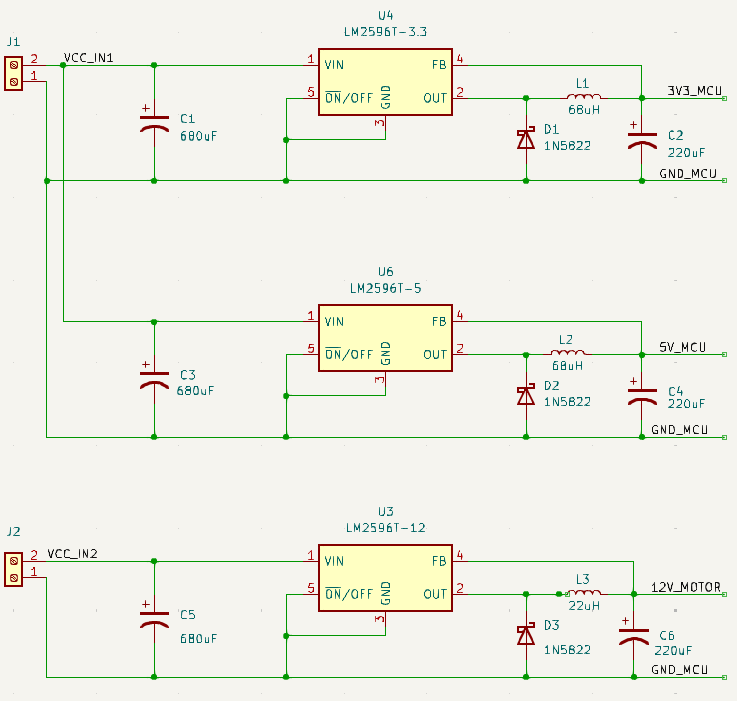
\includegraphics[width=1\textwidth]{pictures/chapter4/c4_p13_PowerSchematic.png}
                    \caption{Sơ đồ nguyên lý mạch nguồn}
                    \label{fig:4-9}
                \end{figure}
                \hspace*{0.6cm}Các linh kiện (điện trở, tụ điện, cuộn cảm) được chọn theo bảng từ tài liệu tham khảo \cite{lm2596}.
                \begin{itemize}
                    \item Với nguồn đầu ra 3.3V, nguồn đầu vào 7.4V và dòng tải không quá 3A, ta chọn: cuộn cảm $L = 22 \mu H$, tụ điện $C_{out} = 680 \mu F$. 
                    \item Với nguồn đầu ra 5V, nguồn đầu vào 7.4V và dòng tải không quá 3A, ta chọn: cuộn cảm $L = 22 \mu H$, tụ điện $C_{out} = 560 \mu F$.
                    \item Với nguồn đầu ra 12V, nguồn đầu vào 14.8V và dòng tải không quá 3A, ta chọn: cuộn cảm $L = 22 \mu H$, tụ điện $C_{out} = 470 \mu F$.
                    \item Chọn tụ điện đầu vào $C_{in} = 680 \mu F, V = 35 V$ cho cả 3 mạch vì $V_{C} = 35 V > 1.5 \times V_{max} = 1.5 \times 14.8 = 22.2 V$.
                \end{itemize}
        \section{Thiết kế mạch cho toàn bộ hệ thống}
            \subsection{Sơ đồ nguyên lý mạch toàn bộ hệ thống}
                \hspace*{0.6cm}Dựa vào các thiết kế mạch cảm biến, mạch nguồn và các linh kiện khác, ta thiết kế sơ đồ nguyên lý mạch toàn bộ hệ thống như sau:
                \begin{figure}[H]
                    \centering
                    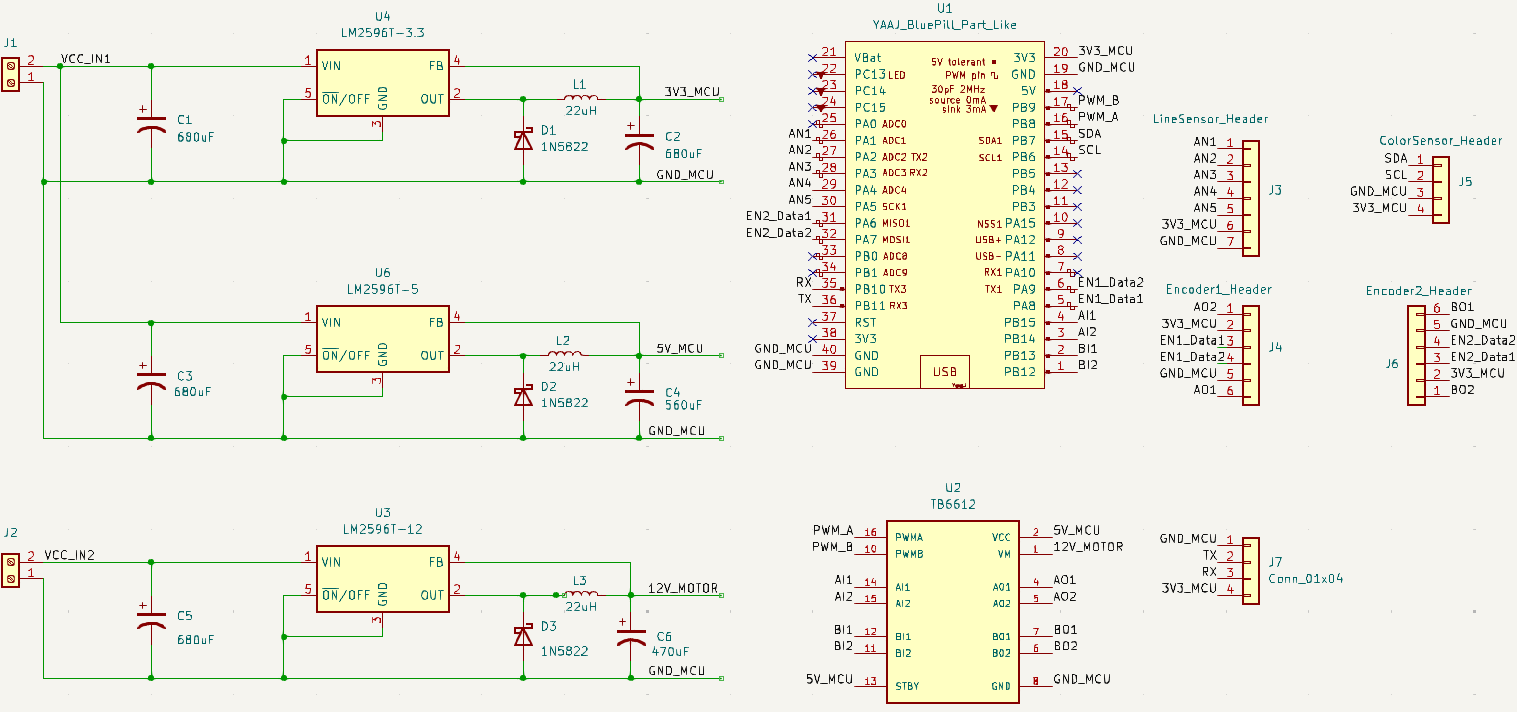
\includegraphics[width=0.95\textwidth]{pictures/chapter4/c4_p14_Schematic.png}
                    \caption{Sơ đồ nguyên lý mạch toàn bộ hệ thống}
                    \label{fig:4-17}
                \end{figure}
            \subsection{Thiết kế PCB mạch toàn bộ hệ thống}
                \hspace*{0.6cm}Dựa vào sơ đồ nguyên lý mạch toàn bộ hệ thống, ta tiến hành thiết kế PCB cho mạch toàn bộ hệ thống. Sơ đồ thiết kế PCB được trình bày như hình \ref{fig:4-18}.
                \begin{figure}[H]
                    \centering
                    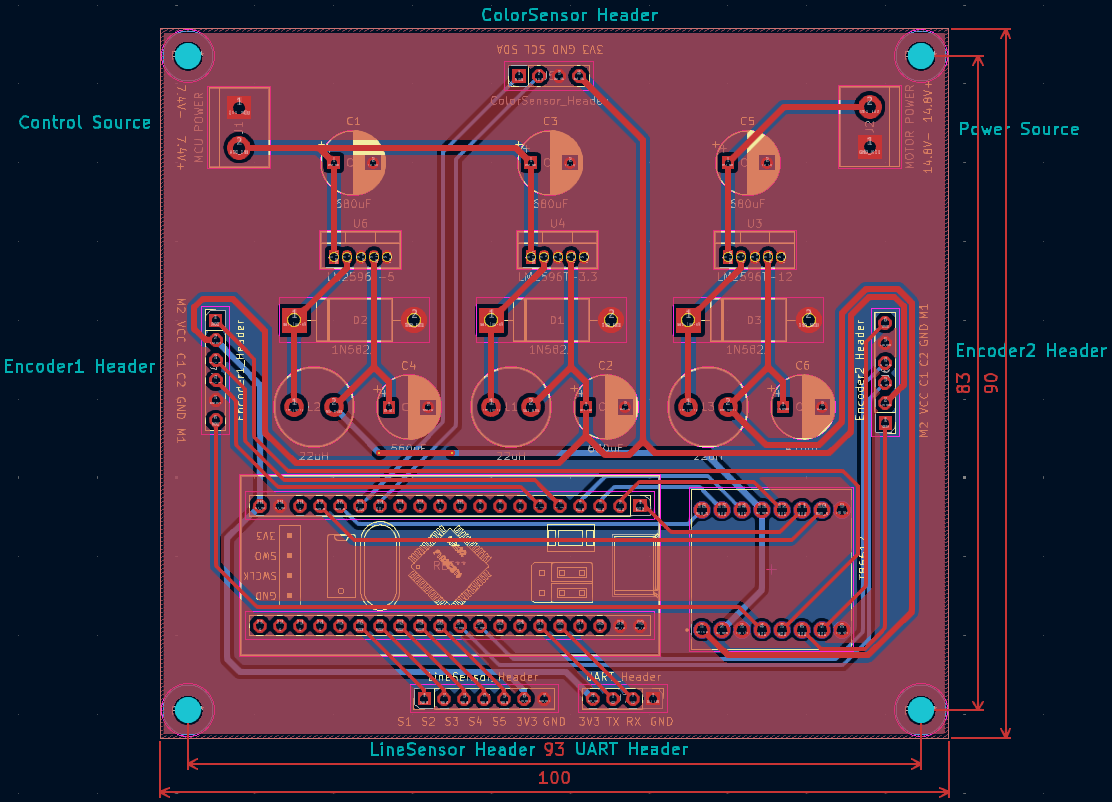
\includegraphics[width=0.8\textwidth]{pictures/chapter4/c4_p15_PCB.png}
                    \caption{Sơ đồ thiết kế PCB mạch toàn bộ hệ thống}
                    \label{fig:4-18}
                \end{figure}
            
                
    \chapter{MÔ HÌNH HÓA}
     \section{Mô hình hóa động học xe dò line}
          \hspace*{0.6cm}Trong chương này, nhóm thực hiện mô hình hóa robot, nhằm mục đích hiểu rõ về cấu trúc của xe, phục vụ cho việc thiết kế bộ điều khiển PID bám line cho xe.
          \newline
          \hspace*{0.6cm}Mục đích của điều khiển các động cơ DC để xe di chuyển bám line trên sa bàn trong điều kiện khá lý tưởng, với tải trọng đặt trên xe là cố định, do đó chương mô hình hóa chỉ tập trung vào xây dựng mô hình động học cho xe mà không quan tâm 
          gì đến mô hình động lực học của xe.
          \begin{figure}[H]
               \centering
               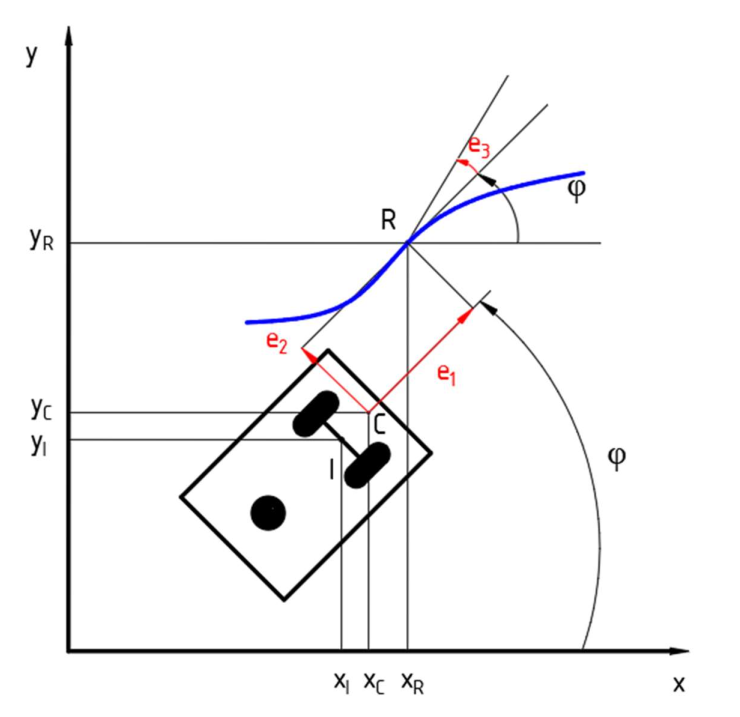
\includegraphics[width=0.7\textwidth]{pictures/chapter5/chapter5_pic1.png}
               \caption{Mô hình động học xe dò line}
               \label{kinematic_model}
          \end{figure}         
          Hình trên mô tả tọa độ các điểm cần thiết của xe trên mặt phẳng tọa độ. Trong đó
          \begin{itemize}
               \item $I(x, y)$: Trung điểm đoạn nối tâm 2 bánh chủ động.
               \item $C(x, y)$: Tâm dãy cảm biến dò line.
               \item $R(x, y)$: Tọa độ điểm tham chiếu trên đường line.
          \end{itemize}
          \hspace*{0.6cm}Phương trình động học tại $I$
          \begin{align*}
               v_{xI} &= \dot{x_I} = v \times \cos \varphi\\
               v_{yI} &= \dot{y_I} = v \times \sin \varphi\\
               \dot{\varphi_I} &= \omega
          \end{align*} 
          Đưa về dạng ma trận
          \begin{align}
               \begin{bmatrix}
                    \dot{x_I} \\
                    \dot{y_I} \\
                    \dot{\varphi_I}
                    \end{bmatrix} &= \begin{bmatrix}
                    \cos\varphi & 0 \\
                    \sin\varphi & 0 \\
                    0 & 1
                    \end{bmatrix} \begin{bmatrix}
                    v \\
                    \omega
               \end{bmatrix}
               \label{c5_e1}
          \end{align}
          \hspace*{0.6cm}Trong đó
          \begin{equation*}
               \begin{cases}
                    v = \dfrac{1}{2}(v_l + v_r) = \dfrac{r\omega_r + r\omega_l}{2} \\[0.5em]
                    \omega = \dfrac{v_r - v_l}{b} = \dfrac{r\omega_r - r\omega_l}{b}
               \end{cases}               
          \end{equation*}
          \begin{itemize}
               \item $v$: vận tốc dài của xe.
               \item $\omega$: vận tốc góc của robot.
               \item $b$: khoảng cách giữa 2 bánh xe.
          \end{itemize}
          \hspace*{0.6cm}Phương trình động học tại điểm bám line $C$
          \begin{equation}
               \begin{cases}
                    x_C = x_I + d \times \cos \varphi \\[0.5em]
                    y_C = y_I + d \times \sin \varphi \\[0.5em]
                    \varphi_C = \varphi_I = \varphi
               \end{cases}   
               \label{c5_e2}            
          \end{equation}
          \hspace*{0.6cm}Lấy đạo hàm ta được 
          \begin{equation}
               \begin{cases}
                    \dot{x_C} = \dot{x_I} - d \times \sin \varphi \dot{\varphi} \\[0.5em]
                    \dot{y_C} = \dot{y_I} + d \times \cos \varphi \dot{\varphi} \\[0.5em]
                    \dot{\varphi_C} = \dot{\varphi_I}
               \end{cases}
               \label{c5_e3}            
          \end{equation}
          \hspace*{0.6cm}Tương tự, mô hình động học tại điểm tham chiếu $R$ trên đường line
          \begin{align}
               \begin{bmatrix}
                    \dot{x_R} \\
                    \dot{y_R} \\
                    \dot{\varphi_R}
                    \end{bmatrix} &= \begin{bmatrix}
                    \cos\varphi_R & 0 \\
                    \sin\varphi_R & 0 \\
                    0 & 1
                    \end{bmatrix} \begin{bmatrix}
                    v_R \\
                    \omega_R
               \end{bmatrix}
               \label{c5_e4}
          \end{align}
          \hspace*{0.6cm}Phương trình biểu diễn sự sai lệch giữa điểm bám line $C$ và vị trí điểm tham chiếu $R$ mong muốn trên đường line
          \begin{equation}
               \begin{cases}
                    x_R - x_C = e_1 \cos \varphi - e_2 \sin \varphi \\[0.5em]
                    y_R - y_C = e_1 \sin \varphi + e_2 \cos \varphi \\[0.5em]
                    \varphi_R - \varphi_C = e_3
               \end{cases}    
               \label{c5_e5}           
          \end{equation}
          \hspace*{0.6cm}Trong đó
          \begin{itemize}
               \item $e_1$: sai số vị trí giữa điểm bám line $C$ và điểm tham chiếu $R$ theo phương vuông góc với trục hai bánh dẫn động.
               \item $e_2$: sai số vị trí giữa điểm bám line $C$ và điểm tham chiếu $R$ theo phương song song với trục hai bánh dẫn động.
               \item $e_3$: sai số góc giữa hướng của xe và hướng tiếp tuyến với sa bàn tại điểm tham chiếu $R$.
          \end{itemize}    
          \hspace*{0.6cm}Từ phương trình (\ref{c5_e5}) rút ra được hệ phương trình các sai số
          \begin{align}
               \begin{bmatrix}
                    e_1 \\
                    e_2 \\
                    e_3
                    \end{bmatrix} &= \begin{bmatrix}
                    \cos\varphi & \sin \varphi & 0 \\
                    -\sin\varphi & \cos \varphi & 0 \\
                    0 & 0 & 1
                    \end{bmatrix} \begin{bmatrix}
                    x_R - x_C \\
                    y_R - y_C \\
                    \varphi_R - \varphi_C
               \end{bmatrix}
               \label{c5_e6}
          \end{align}
          \hspace*{0.6cm}Đạo hàm 2 vế hệ (\ref{c5_e6}), khai triển và rút gọn ta thu được 
          \begin{align}
               \begin{bmatrix}
                    \dot{e_1} \\
                    \dot{e_2} \\
                    \dot{e_3}
                    \end{bmatrix} &= \begin{bmatrix}
                    v_R \cos e_3 \\
                    v_R \sin e_3 \\
                    \omega_R
                    \end{bmatrix} + \begin{bmatrix}
                    -1 & e_2 \\
                    0 & -d - e_1 \\
                    0 & -1
                    \end{bmatrix} \begin{bmatrix}
                    v_I \\
                    \omega_I
               \end{bmatrix}
               \label{c5_e7}
          \end{align}       
     \section{Tính toán thời gian lấy mẫu}
          \subsection{Tính toán thời gian lấy mẫu cho bộ điều khiển động cơ}
               \hspace*{0.6cm}Nhóm cần tính toán thời gian lấy mẫu cho động cơ \textit{JGB37-520 333RPM} có gắn encoder với các thông số như số vòng quay sau 
               hộp giảm tốc là 333 vòng/phút, 2 kênh encoder với mỗi kênh nhận 11 xung/vòng.\\
               Số vòng quay tối đa của động cơ
               \begin{equation*}
                    333 \,\mathrm{rpm} = \dfrac{333}{60} \,\mathrm{rev/s} = 5.55 \,\mathrm{rev/s}
               \end{equation*}
               Sử dụng 2 kênh encoder với chế độ quadrature, nghĩa là mỗi vòng encoder đếm tổng cộng $11 \times 4 = 44 \,\mathrm{xung}$.\\
               Tần số xung và thời gian giữa 2 lần đếm xung của encoder là 
               \begin{align*}
                    &f_{\text{pulse}} = 44 \times 5.55 = 244.2 \,\mathrm{Hz}\\
                    &T_{\text{pulse}} = \dfrac{1}{244.2} = 4.095 \,\mathrm{ms}
               \end{align*}
               Sử dụng tiêu chuẩn Nyquist, tần số tối thiểu (tương đương với thời gian lấy mẫu tối da để khôi phục tín hiệu xung) là 
               \begin{align*}
                    &f_s \geq 2 f_{\text{pulse}} = 2 \time 244.2 = 488.4 \,\mathrm{Hz}\\
                    &t_s \leq \dfrac{1}{f_s} = \dfrac{1}{488.4} = 2.05 \,\mathrm{ms}
               \end{align*}
               Nếu lấy mẫu theo tiêu chuẩn Nyquist, số lượng xung ở mỗi lần lấy mẫu không đủ, nhiều mẫu bị mất xung, nhóm sử dụng chế độ Encoder Mode của STM32 để tính toán
               số xung encoder trong mỗi lần ngắt để tính toán tốc độ động cơ làm giá trị phản hồi cho vòng điều khiển, do đó cần lựa chọn khoảng thời gian lấy mẫu sao cho số xung đọc được 
               ổn định để tính toán giá trị vận tốc động cơ. Số xung mà vi điều khiển đọc được trong khoảng thời gian lấy mẫu $t_s$ là 
               \begin{equation*}
                    n = \dfrac{t_s}{T_{\text{pulse}}} = \dfrac{t_s}{4.095}
               \end{equation*}
               Nhóm lựa chọn thời gian lấy mẫu cho bộ điều khiển tốc độ động cơ là $t_s = 0.01 \,\mathrm{s}$.
          \subsection{Tính toán thời gian lấy mẫu cho bộ điều khiển bám line}
               \hspace*{0.6cm}Để tính toán thời gian lấy mẫu cho bộ điều khiển bám line, ta tính toán quãng đường tối đa mà xe di chuyển trên đoạn đường cong 
               có bán kính lớn nhất trong khoảng thời gian giữa 2 lần lấy mẫu mà vẫn đảm bảo được sai số bám line.\\
               \hspace*{0.6cm}Giả sử tâm cảm biến dò line nằm ngay tại vị trí tâm đường line tại thời điểm đầu, tại thời điểm lấy mẫu kế tiếp, với mong muốn sai số $e_2$ giữa tâm đường cảm biến 
               và tâm line không lệch nhau quá 3mm. Do đó quãng đường AB lớn nhất mà xe chạy được trước khi đạt tới sai số 3mm là 
               \begin{equation*}
                    AB = \sqrt{OB^2 - OA^2} = \sqrt{(OA + e_{2max})^2 - OA^2}
               \end{equation*}
               Trong đó 
               \begin{itemize}
                    \item $OA$ là bán kính của đường cong.
                    \item $e_{2max}$ là khoảng sai số lớn nhất khi di chuyển trên cung.
               \end{itemize}
               Ta thấy khi $OA$ càng lớn thì khoảng di chuyển trên cung của xe càng lớn, ta tính toán với bán kính $OA = 800 \,\mathrm{mm}$
               \begin{equation*}
                    AB = 69.34 \,\mathrm{mm}
               \end{equation*}
               Để xe có thể bám được line khi vào đoạn đường cong trên thì thời gian lấy mẫu cho bộ điều khiển vị trí bám line phải thỏa
               \begin{equation*}
                    t_{\text{đk}} \leq \dfrac{AB}{v} = \dfrac{69.34}{300} = 0.23 \,\mathrm{s}
               \end{equation*}
               $v$ là vận tốc của xe khi vào cua: $v = 300 \,\mathrm{mm/s}$.
               Ta chọn $t_{\text{đk}} = 0.05 \,\mathrm{s}$.

     \section{Mô hình hóa động cơ}
          \hspace*{0.6cm}Thực hiện mô hình hóa động cơ, tìm hàm truyền động cơ bằng cách xem xét mối quan hệ giữa đầu vào giá xung PWM và đầu ra là tốc độ quay của trục động cơ (vòng/phút).   
          \subsection{Mô hình hóa động cơ dẫn động bánh phải}    
               \hspace*{0.6cm}Sử dụng driver TB6612FNG, sau khi cấp xung và đo tốc độ động cơ, thu được bảng số liệu sau
               \begin{table}[h!]
                    \centering
                    \begin{tabular}{|c|c|}
                         \hline
                         \textbf{\%PWM} & \textbf{RPM} \\
                         \hline
                         0 & 0 \\
                         5 & 0 \\
                         10 & 0 \\
                         15 & 9.0909 \\
                         20 & 22.7273 \\
                         25 & 45.4545 \\
                         30 & 63.6364 \\
                         35 & 77.2727 \\
                         40 & 95.4545 \\
                         45 & 109.0909 \\
                         50 & 122.7273 \\
                         55 & 131.8182 \\
                         60 & 154.5455 \\
                         65 & 172.7273 \\
                         70 & 181.8182 \\
                         75 & 195.4545 \\
                         80 & 209.0909 \\
                         85 & 227.2727 \\
                         90 & 236.3636 \\
                         95 & 254.5454 \\
                         100 & 263.6364 \\
                         95 & 268.1818 \\
                         90 & 263.6364 \\
                         85 & 250.0000 \\
                         80 & 240.9091 \\
                         75 & 231.8182 \\
                         70 & 218.1818 \\
                         65 & 204.5455 \\
                         60 & 186.3636 \\
                         55 & 177.2727 \\
                         50 & 154.5455 \\
                         45 & 140.9091 \\
                         40 & 136.3636 \\
                         35 & 127.2727 \\
                         30 & 100.0000 \\
                         25 & 86.3636 \\
                         20 & 63.6364 \\
                         15 & 45.4545 \\
                         10 & 36.3636 \\
                         5 & 22.7273 \\
                         0 & 0 \\
                         \hline
                    \end{tabular}
                    \caption{Quan hệ giữa \%PWM và tốc độ quay (RPM)}
               \end{table}
               \newpage
               \hspace*{0.6cm}Đáp ứng của động cơ bánh phải theo thời gian
               \begin{figure}[H]
                    \centering
                    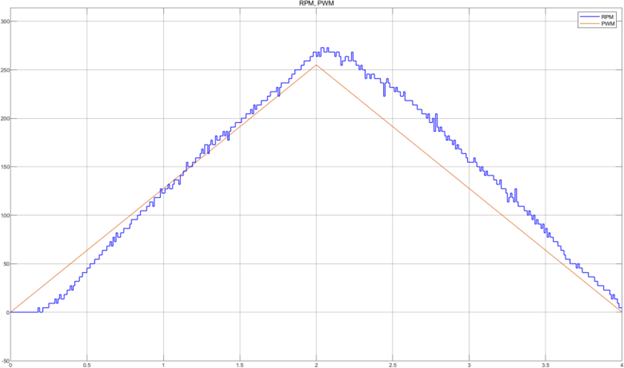
\includegraphics[width=1\textwidth]{pictures/chapter5/CJGB1_response.png}
                    \caption{Đáp ứng của động cơ bánh phải}
                    \label{CJGB1_response}
               \end{figure}  
               \hspace*{0.6cm}Sử dụng Toolbox System Identification của Matlab ta có hàm truyền của động cơ bánh phải 
               \begin{figure}[H]
                    \centering
                    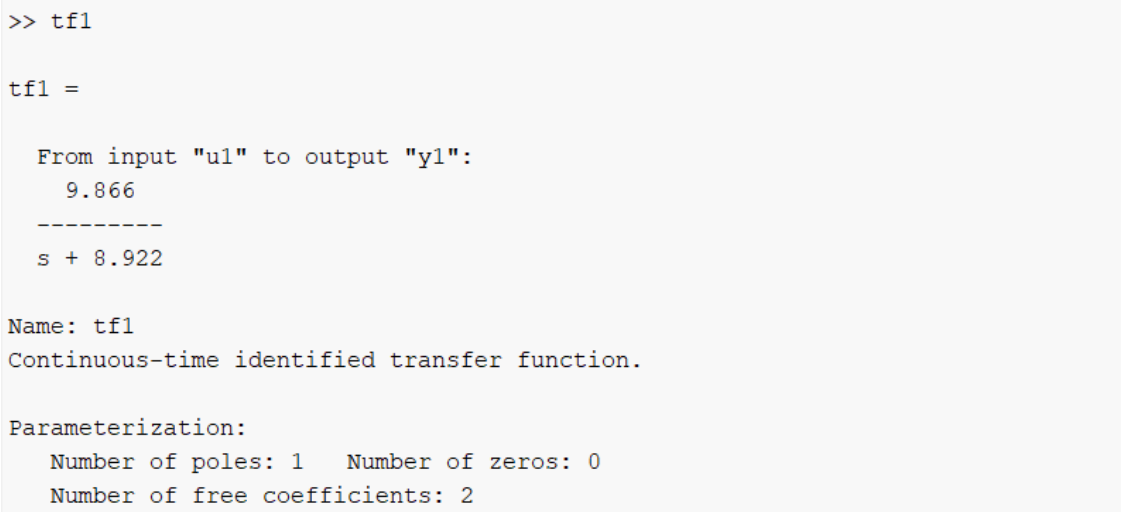
\includegraphics[width=1\textwidth]{pictures/chapter5/CJGB1_tf.png}
                    \caption{Hàm truyền động cơ bánh phải}
                    \label{CJGB1_tf}
               \end{figure} 
               \hspace*{0.6cm}So sánh giữa đáp ứng thực tế và hàm truyền của động cơ bánh phải
               \begin{figure}[H]
                    \centering
                    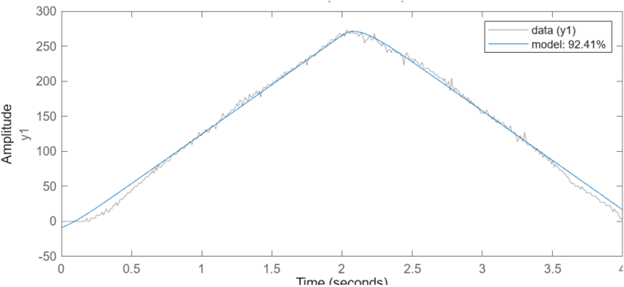
\includegraphics[width=1\textwidth]{pictures/chapter5/CJGB1_compare.png}
                    \caption{Hàm truyền động cơ bánh phải}
                    \label{CJGB1_compare}
               \end{figure} 
          \subsection{Mô hình hóa động cơ dẫn động bánh trái}
               \hspace*{0.6cm}Tương tự như thu thập dữ liệu bánh phải động cơ, sau khi cấp xung và đo tốc độ động cơ, thu được bảng số liệu sau
               \begin{table}[h!]
                    \centering
                    \begin{tabular}{|c|c|}
                         \hline
                         \textbf{\%PWM} & \textbf{RPM} \\
                         \hline
                         0   & 0 \\
                         5   & 4.55 \\
                         10  & 0 \\
                         15  & 18.18 \\
                         20  & 31.82 \\
                         25  & 50.00 \\
                         30  & 59.09 \\
                         35  & 63.64 \\
                         40  & 100.00 \\
                         45  & 122.73 \\
                         50  & 145.45 \\
                         55  & 145.45 \\
                         60  & 159.09 \\
                         65  & 163.64 \\
                         70  & 186.36 \\
                         75  & 200.00 \\
                         80  & 218.18 \\
                         85  & 231.82 \\
                         90  & 245.45 \\
                         95  & 272.73 \\
                         100 & 277.27 \\
                         95  & 281.82 \\
                         90  & 259.09 \\
                         85  & 268.18 \\
                         80  & 245.45 \\
                         75  & 240.91 \\
                         70  & 222.73 \\
                         65  & 204.55 \\
                         60  & 190.91 \\
                         55  & 181.82 \\
                         50  & 150.00 \\
                         45  & 150.00 \\
                         40  & 122.73 \\
                         35  & 109.09 \\
                         30  & 100.00 \\
                         25  & 90.91 \\
                         20  & 63.64 \\
                         15  & 45.45 \\
                         10  & 31.82 \\
                         5   & 27.27 \\
                         0   & 9.09 \\
                         \hline
                    \end{tabular}
                    \caption{Quan hệ giữa \%PWM và tốc độ quay (RPM)}
               \end{table}
               \newpage
               \hspace*{0.6cm}Đáp ứng của động cơ bánh trái theo thời gian
               \begin{figure}[H]
                    \centering
                    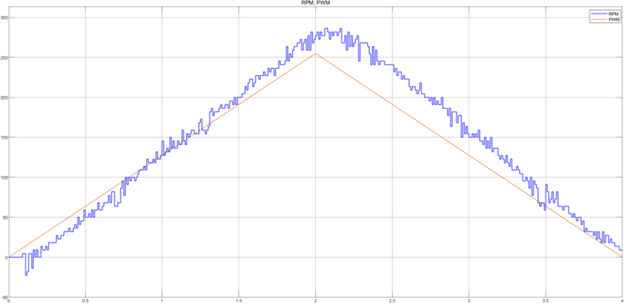
\includegraphics[width=1\textwidth]{pictures/chapter5/CJGB2_response.png}
                    \caption{Đáp ứng của động cơ bánh trái}
                    \label{CJGB2_response}
               \end{figure}  
               \hspace*{0.6cm}Sử dụng Toolbox System Identification của Matlab ta có hàm truyền của động cơ bánh trái 
               \begin{figure}[H]
                    \centering
                    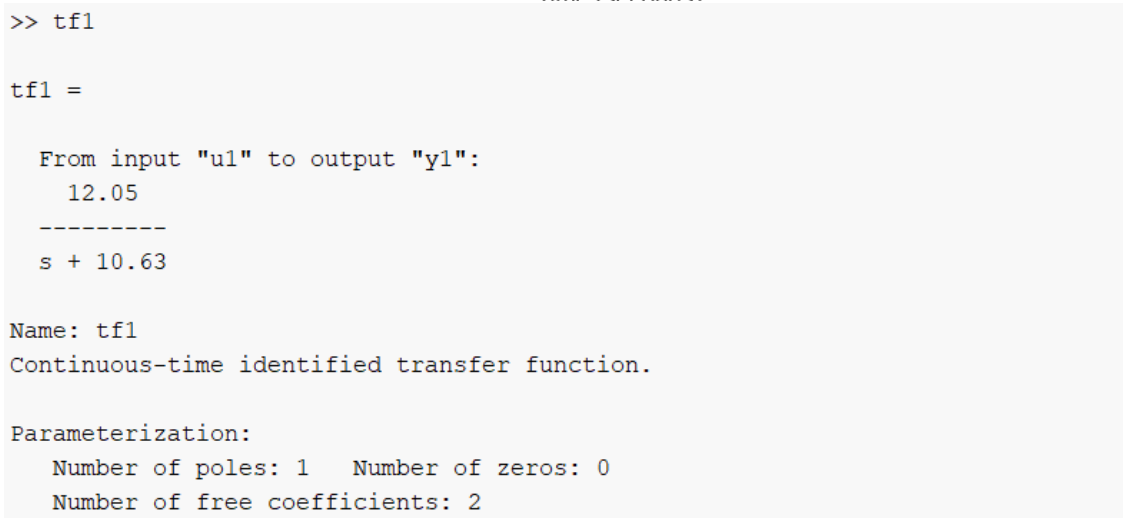
\includegraphics[width=1\textwidth]{pictures/chapter5/CJGB2_tf.png}
                    \caption{Hàm truyền động cơ bánh trái}
                    \label{CJGB2_tf}
               \end{figure} 
               \hspace*{0.6cm}So sánh giữa đáp ứng thực tế và hàm truyền của động cơ bánh trái
               \begin{figure}[H]
                    \centering
                    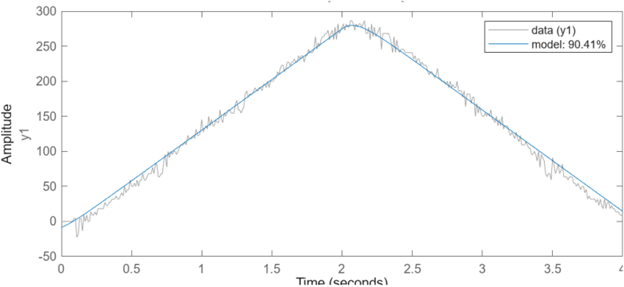
\includegraphics[width=1\textwidth]{pictures/chapter5/CJGB2_compare.png}
                    \caption{Hàm truyền động cơ bánh trái}
                    \label{CJGB2_compare}
               \end{figure}
     




          



    \chapter{THIẾT KẾ GIẢI THUẬT ĐIỀU KHIỂN}
     \section{Giải thuật bám line}
          \hspace*{0.6cm}Bộ điều khiển giúp xe bám line bằng cách giảm thiểu sai số $e$ nhỏ nhất có thể thông qua điều khiển tốc độ 2 động cơ DC. Bộ điều khiển PID được lựa chọn cho bài toán bám line.
          \newline
          \hspace*{0.6cm}Xác định đầu vào và đầu ra của bộ điều khiển
          \begin{itemize}
               \item Input: sai số giữa điểm bám line $C$ và điểm tham chiếu $R$ trên đường line.
               \item Output: Tốc độ góc của hai bánh xe.
          \end{itemize}
          \hspace*{0.6cm}Từ chương 5 mô hình hóa ta có
          \begin{align}
               \begin{bmatrix}
                    e_1 \\
                    e_2 \\
                    e_3
                    \end{bmatrix} &= \begin{bmatrix}
                    \cos\varphi & \sin \varphi & 0 \\
                    -\sin\varphi & \cos \varphi & 0 \\
                    0 & 0 & 1
                    \end{bmatrix} \begin{bmatrix}
                    x_R - x_C \\
                    y_R - y_C \\
                    \varphi_R - \varphi_C
               \end{bmatrix} 
               \label{c6_e1}
          \end{align}
          \begin{align}
               \begin{bmatrix}
                    \dot{e_1} \\
                    \dot{e_2} \\
                    \dot{e_3}
                    \end{bmatrix} &= \begin{bmatrix}
                    v_R \cos e_3 \\
                    v_R \sin e_3 \\
                    \omega_R
                    \end{bmatrix} + \begin{bmatrix}
                    -1 & e_2 \\
                    0 & -d - e_1 \\
                    0 & -1
                    \end{bmatrix} \begin{bmatrix}
                    v_I \\
                    \omega_I
               \end{bmatrix}  
               \label{c6_e2}             
          \end{align}
          \hspace*{0.6cm}Hệ được mô tả bởi không gian trạng thái
          \begin{equation}
               \dot{x} = Ax + Bu 
               \label{c6_e3}
          \end{equation}
          \hspace*{0.6cm}Trong đó
          \begin{equation*}
               \dot{x} = \begin{bmatrix}
                    \dot{e_1} \\
                    \dot{e_2} \\
                    \dot{e_3}
               \end{bmatrix};
               x = \begin{bmatrix}
                    e_1 \\
                    e_2 \\
                    e_3
               \end{bmatrix}; 
               u = \begin{bmatrix}
                    v \\ 
                    \omega
               \end{bmatrix}
          \end{equation*}
          \hspace{0.6cm}Nhận thấy điểm cân bằng của hệ phi tuyến là $X_0 = [e_{10} \, e_{20} \, e_{30}] = [0 \, 0 \, 0]^{\text{T}}$. Phân tích và tuyến tính hóa hệ quanh điểm cân bằng ta tính được các ma trận
          \begin{equation*}
               A = \begin{bmatrix}
               0 & \omega & -v_R \times \sin e_3 \\
               -\omega & 0 & v_R \times \cos e_3 \\
               0 & 0 & 0
               \end{bmatrix}; \quad B = \begin{bmatrix}
               -1 & e_2 \\
               0 & -d - e_1 \\
               0 & -1
               \end{bmatrix}
          \end{equation*}
          Suy ra 
          \begin{align}
               \begin{bmatrix}
               \dot{e}_1 \\
               \dot{e}_2 \\
               \dot{e}_3
               \end{bmatrix} &= \begin{bmatrix}
               0 & \omega & -v_R \times \sin e_3 \\
               -\omega & 0 & v_R \times \cos e_3 \\
               0 & 0 & 0
               \end{bmatrix} \begin{bmatrix}
               e_1 \\
               e_2 \\
               e_3
               \end{bmatrix} + \begin{bmatrix}
               -1 & e_2 \\
               0 & -d - e_1 \\
               0 & -1
               \end{bmatrix} \begin{bmatrix}
               v \\
               \omega
               \end{bmatrix}\\
               &\approx \begin{bmatrix}
               0 & \omega & 0 \\
               -\omega & 0 & v_R \\
               0 & 0 & 0
               \end{bmatrix} \begin{bmatrix}
               e_1 \\
               e_2 \\
               e_3
               \end{bmatrix} + \begin{bmatrix}
               -1 & 0 \\
               0 & -d \\
               0 & -1
               \end{bmatrix} \begin{bmatrix}
               v \\
               \omega
               \end{bmatrix}
               \label{c6_e4}
          \end{align}
          


\end{document}